\chapter{Appendix}\label{chap:appendix}
\section{Simulations with base 10}
\subsection{Complete Graph}
\begin{figure}[H]
    \centering
    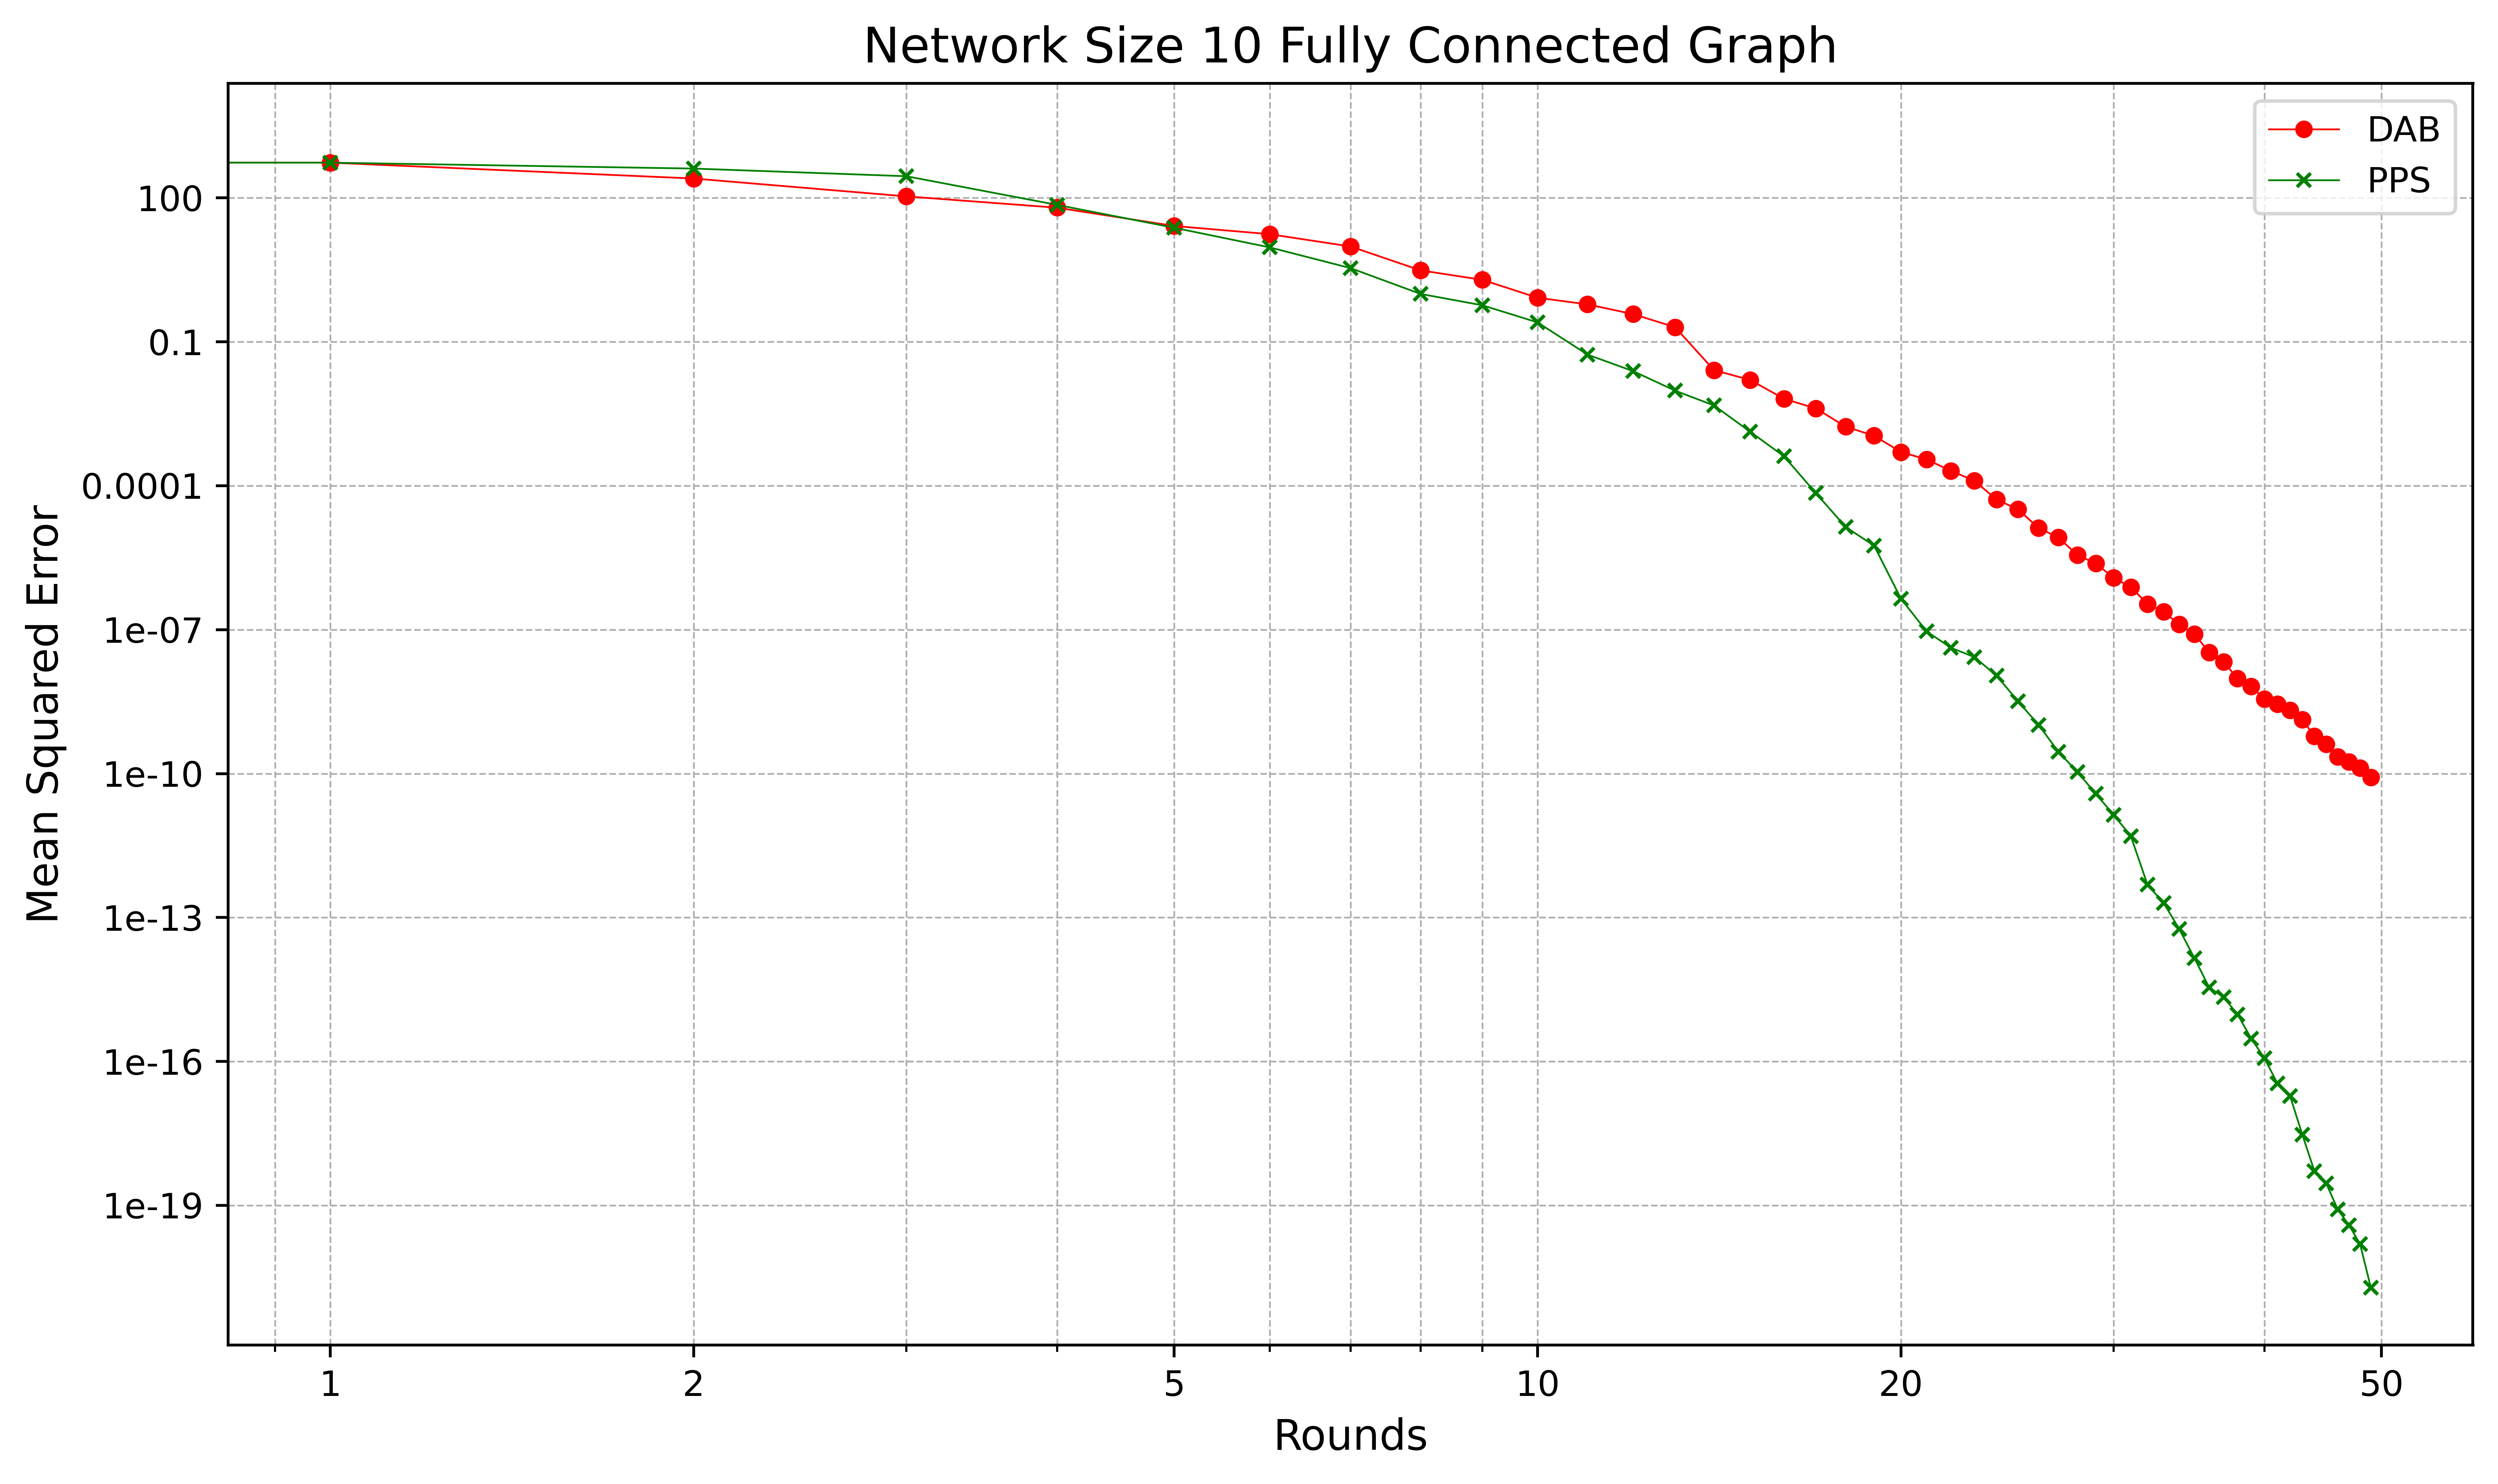
\includegraphics[scale=0.5]{figures/completeGraphSimulations/DAB_vs_PPS_FCG_r50_n10.png}
    \caption{Fully connected graph: network size $10^{1}$ nodes}
    \label{fig:10CompleteGraph}
\end{figure}
\begin{figure}[H]
    \centering
    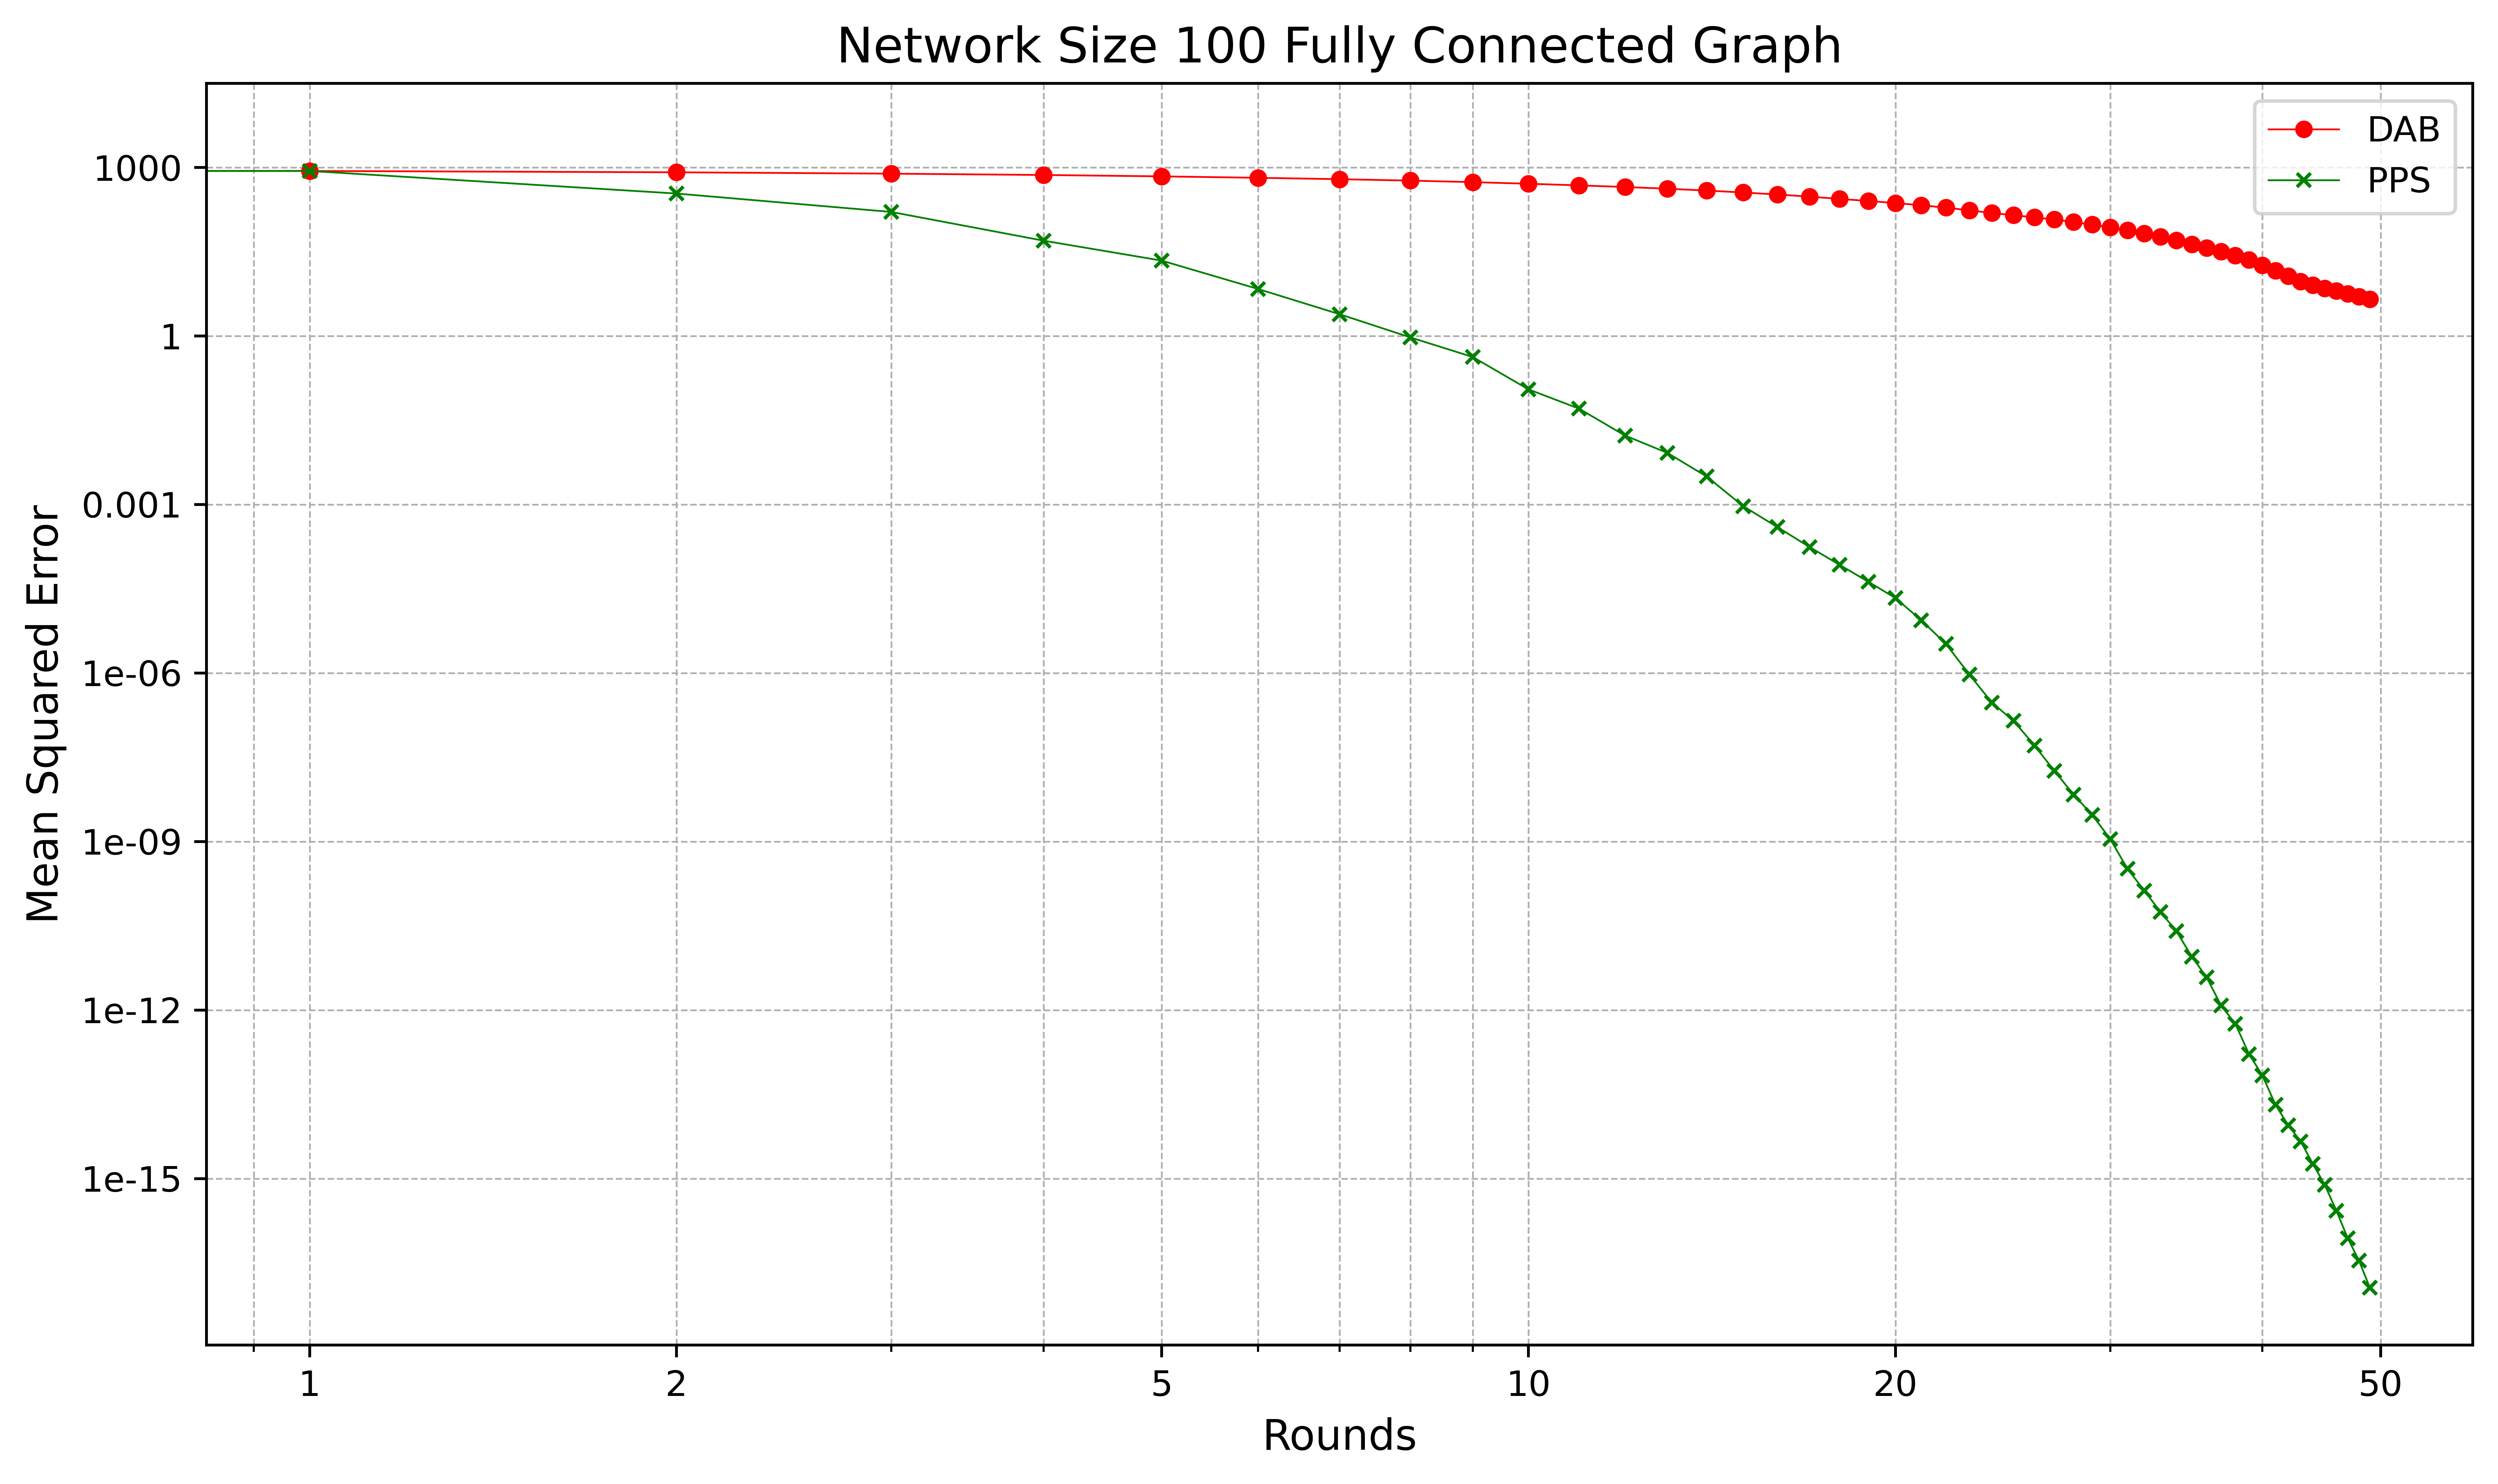
\includegraphics[scale=0.5]{figures/completeGraphSimulations/DAB_vs_PPS_FCG_r50_n100.png}
    \caption{Fully connected graph: network size $10^{2}$ nodes}
    \label{fig:100CompleteGraph}
\end{figure}
\begin{figure}[H]
    \centering
    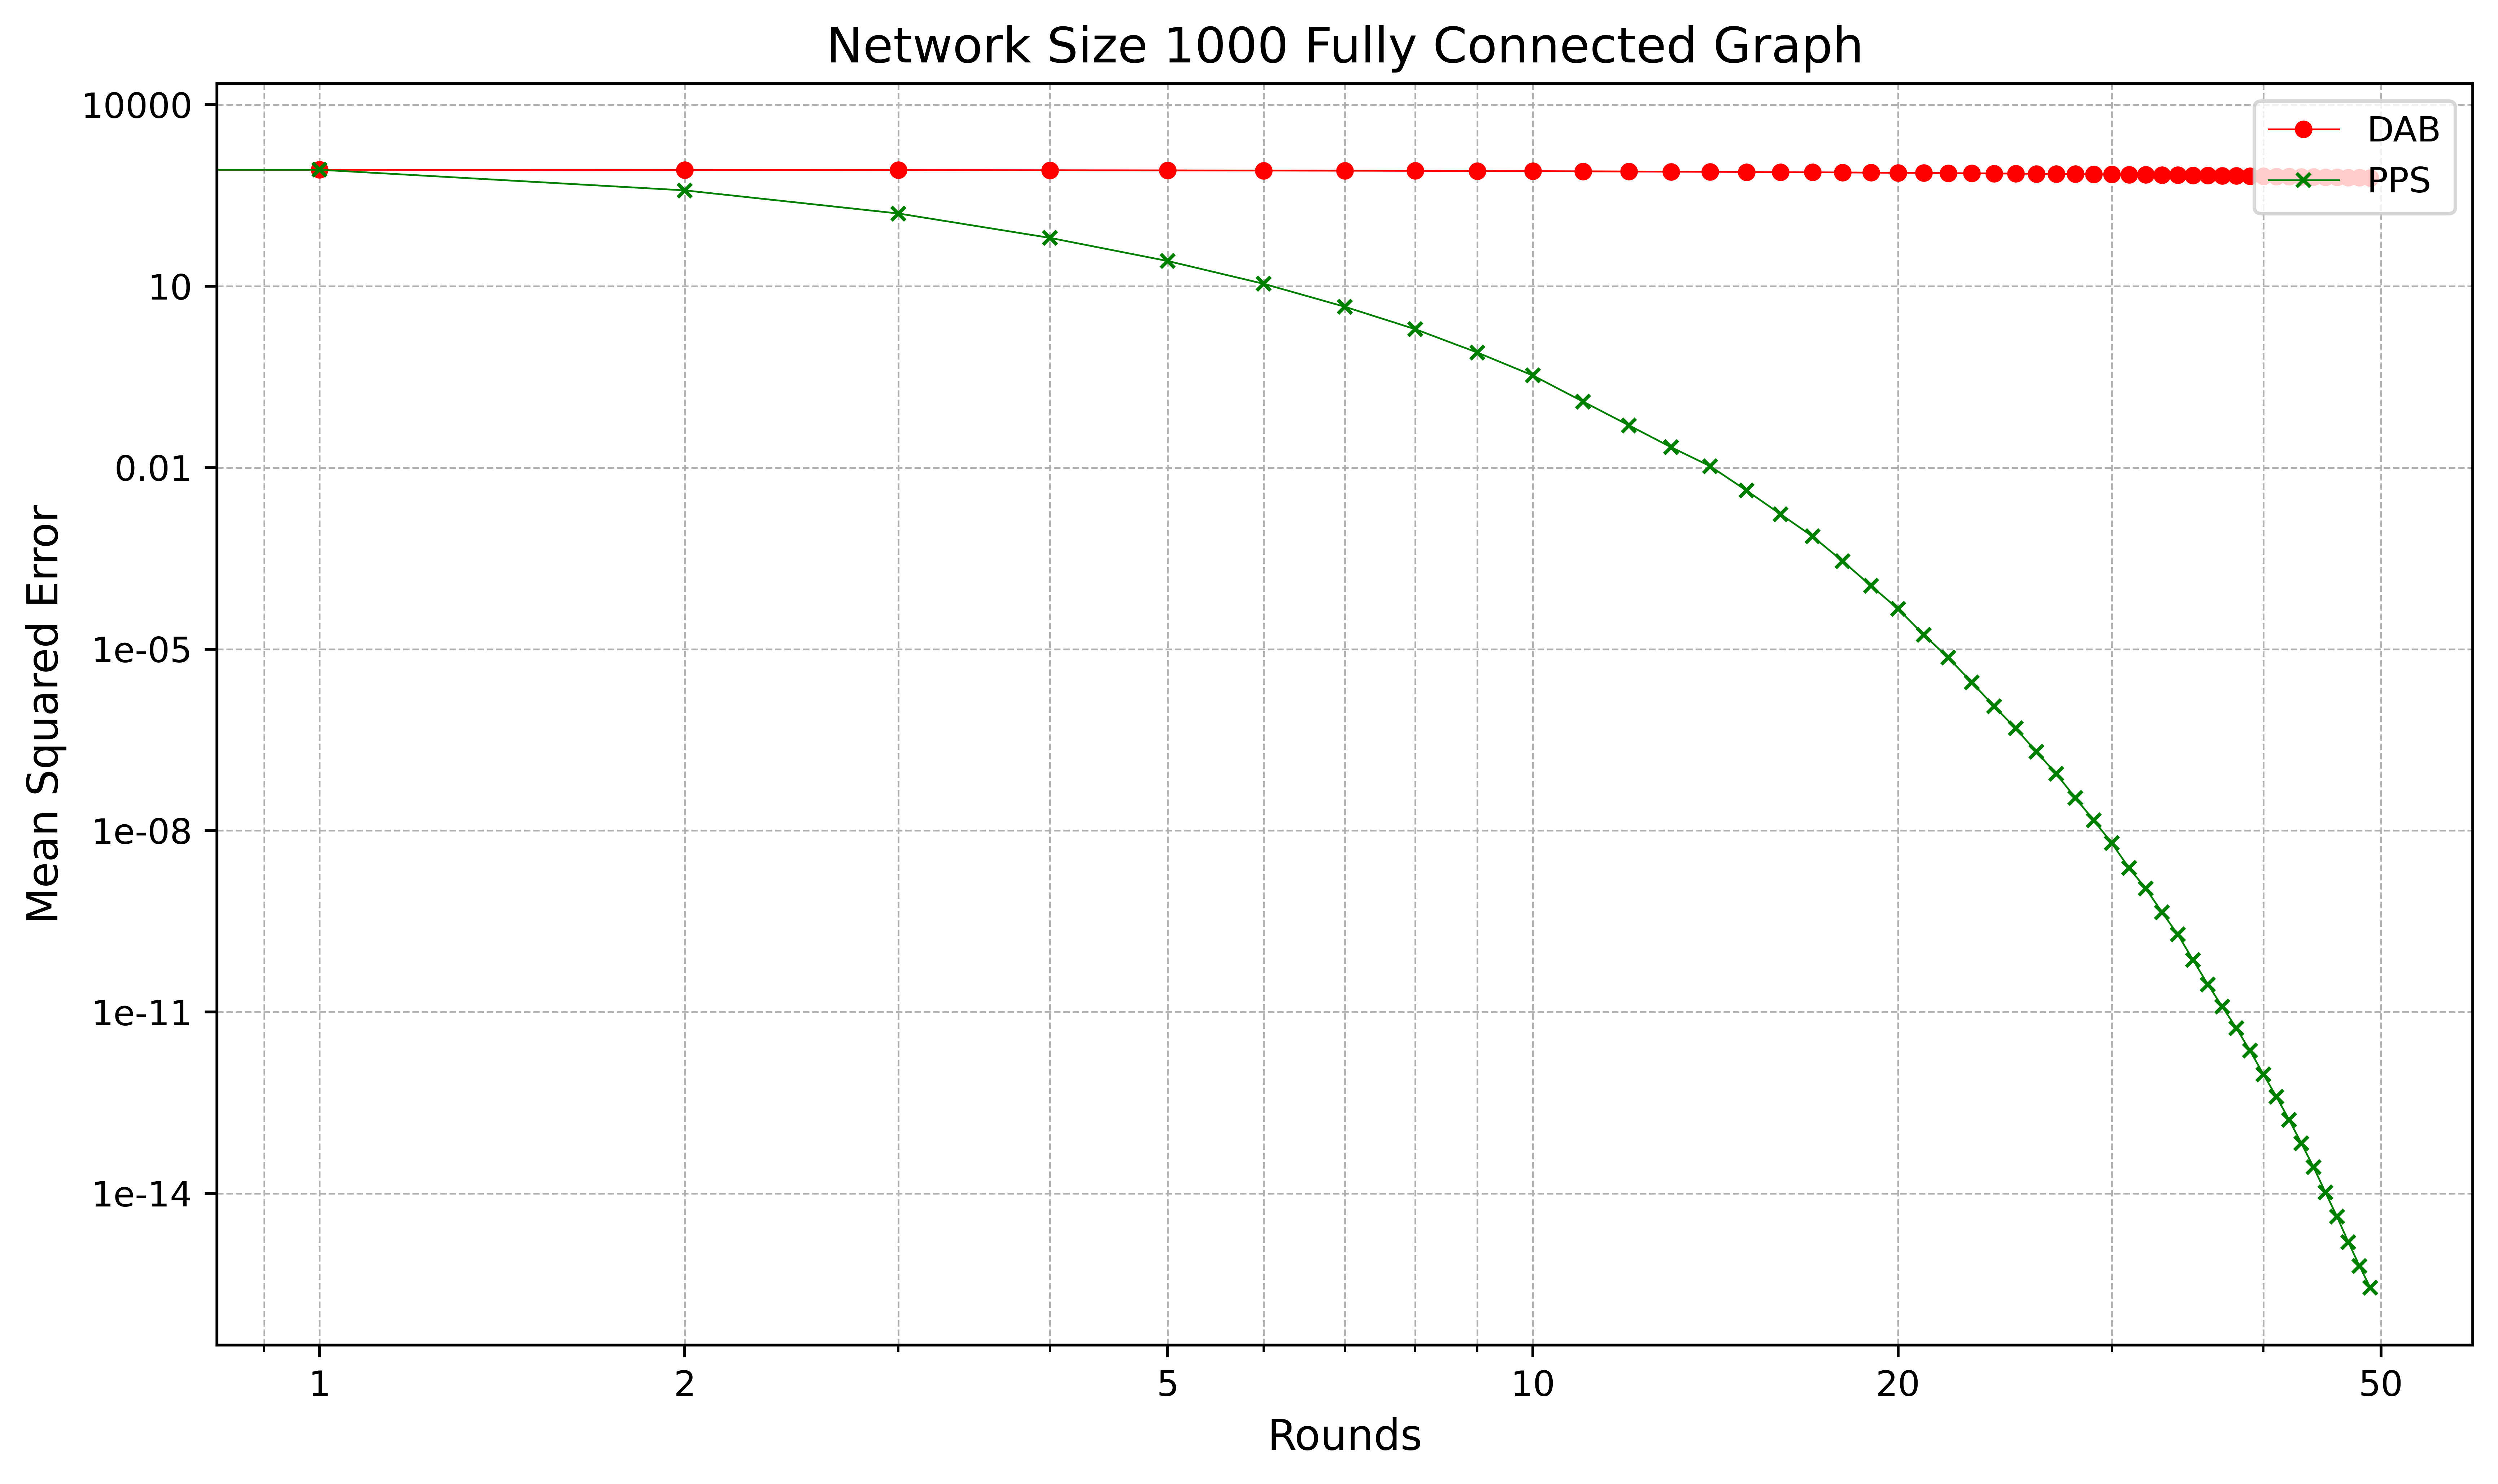
\includegraphics[scale=0.5]{figures/completeGraphSimulations/DAB_vs_PPS_FCG_r50_n1000.png}
    \caption{Fully connected graph: network size $10^{3}$ nodes}
    \label{fig:1000CompleteGraph}
\end{figure}
\begin{figure}[H]
    \centering
    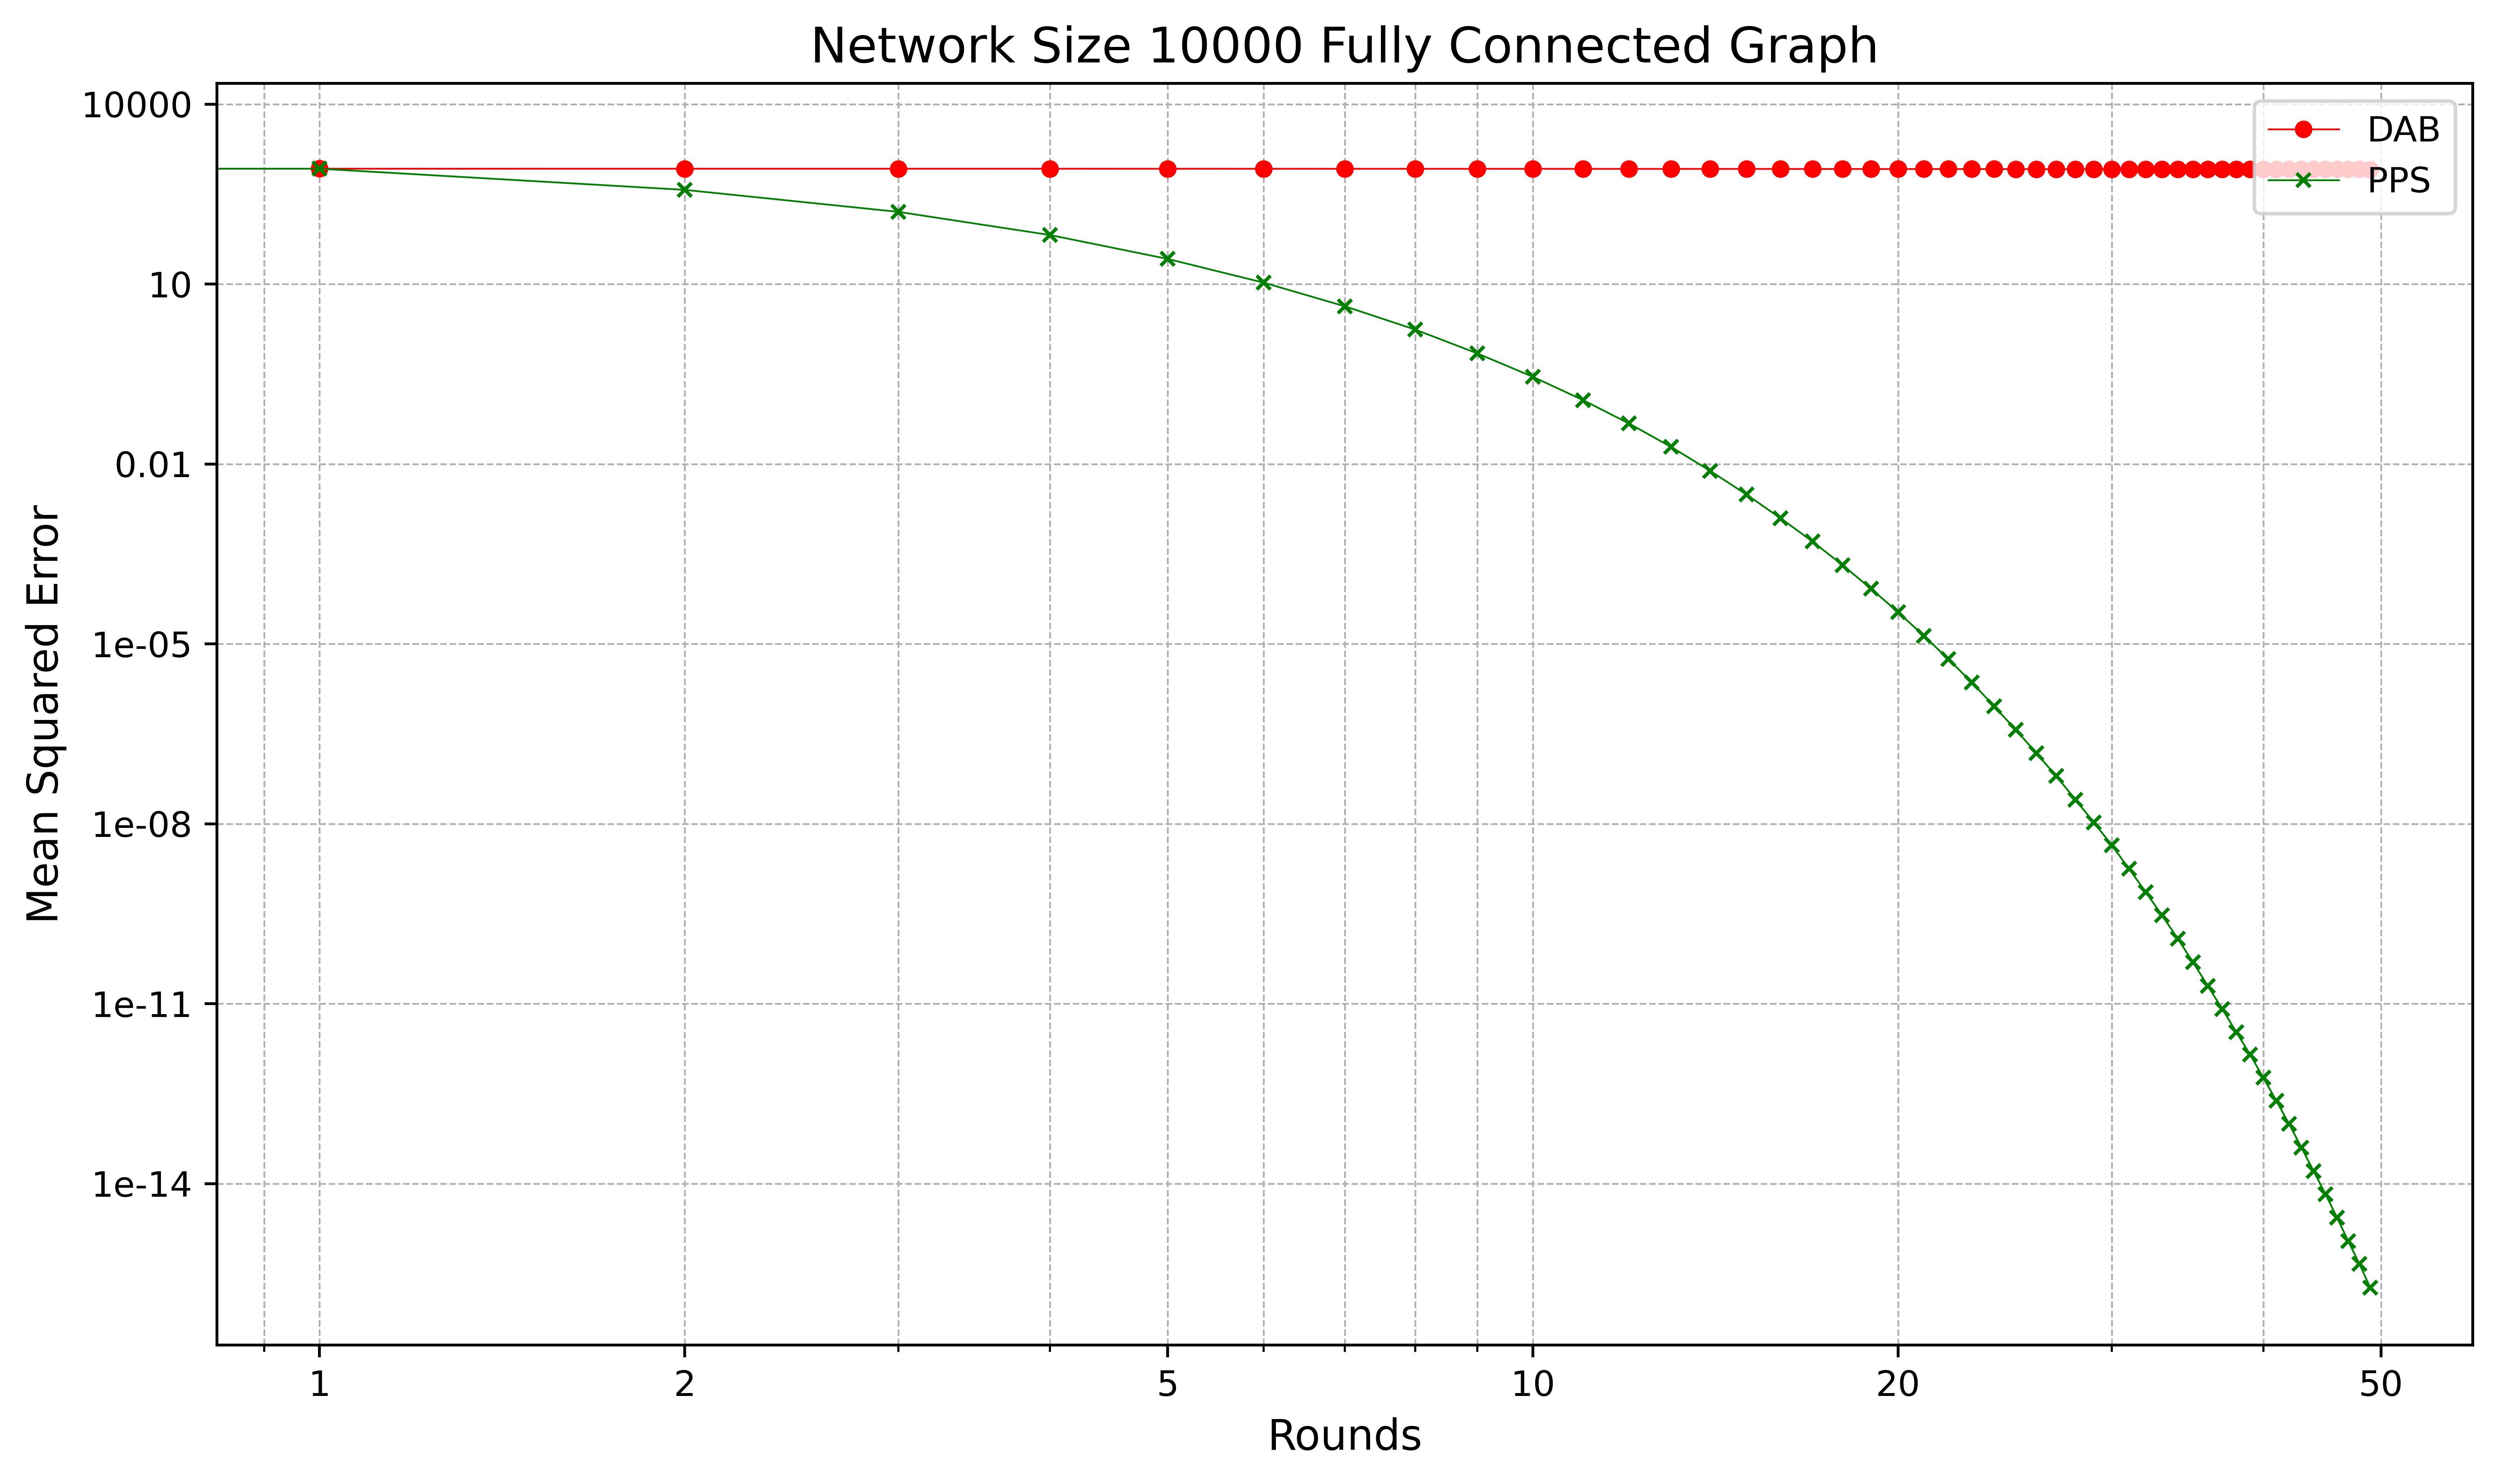
\includegraphics[scale=0.5]{figures/completeGraphSimulations/DAB_vs_PPS_FCG_r50_n10000.png}
    \caption{Fully connected graph: network size $10^{4}$ nodes}
    \label{fig:10000CompleteGraph}
\end{figure}

\subsection{Star Graph}
\begin{figure}[H]
    \centering
    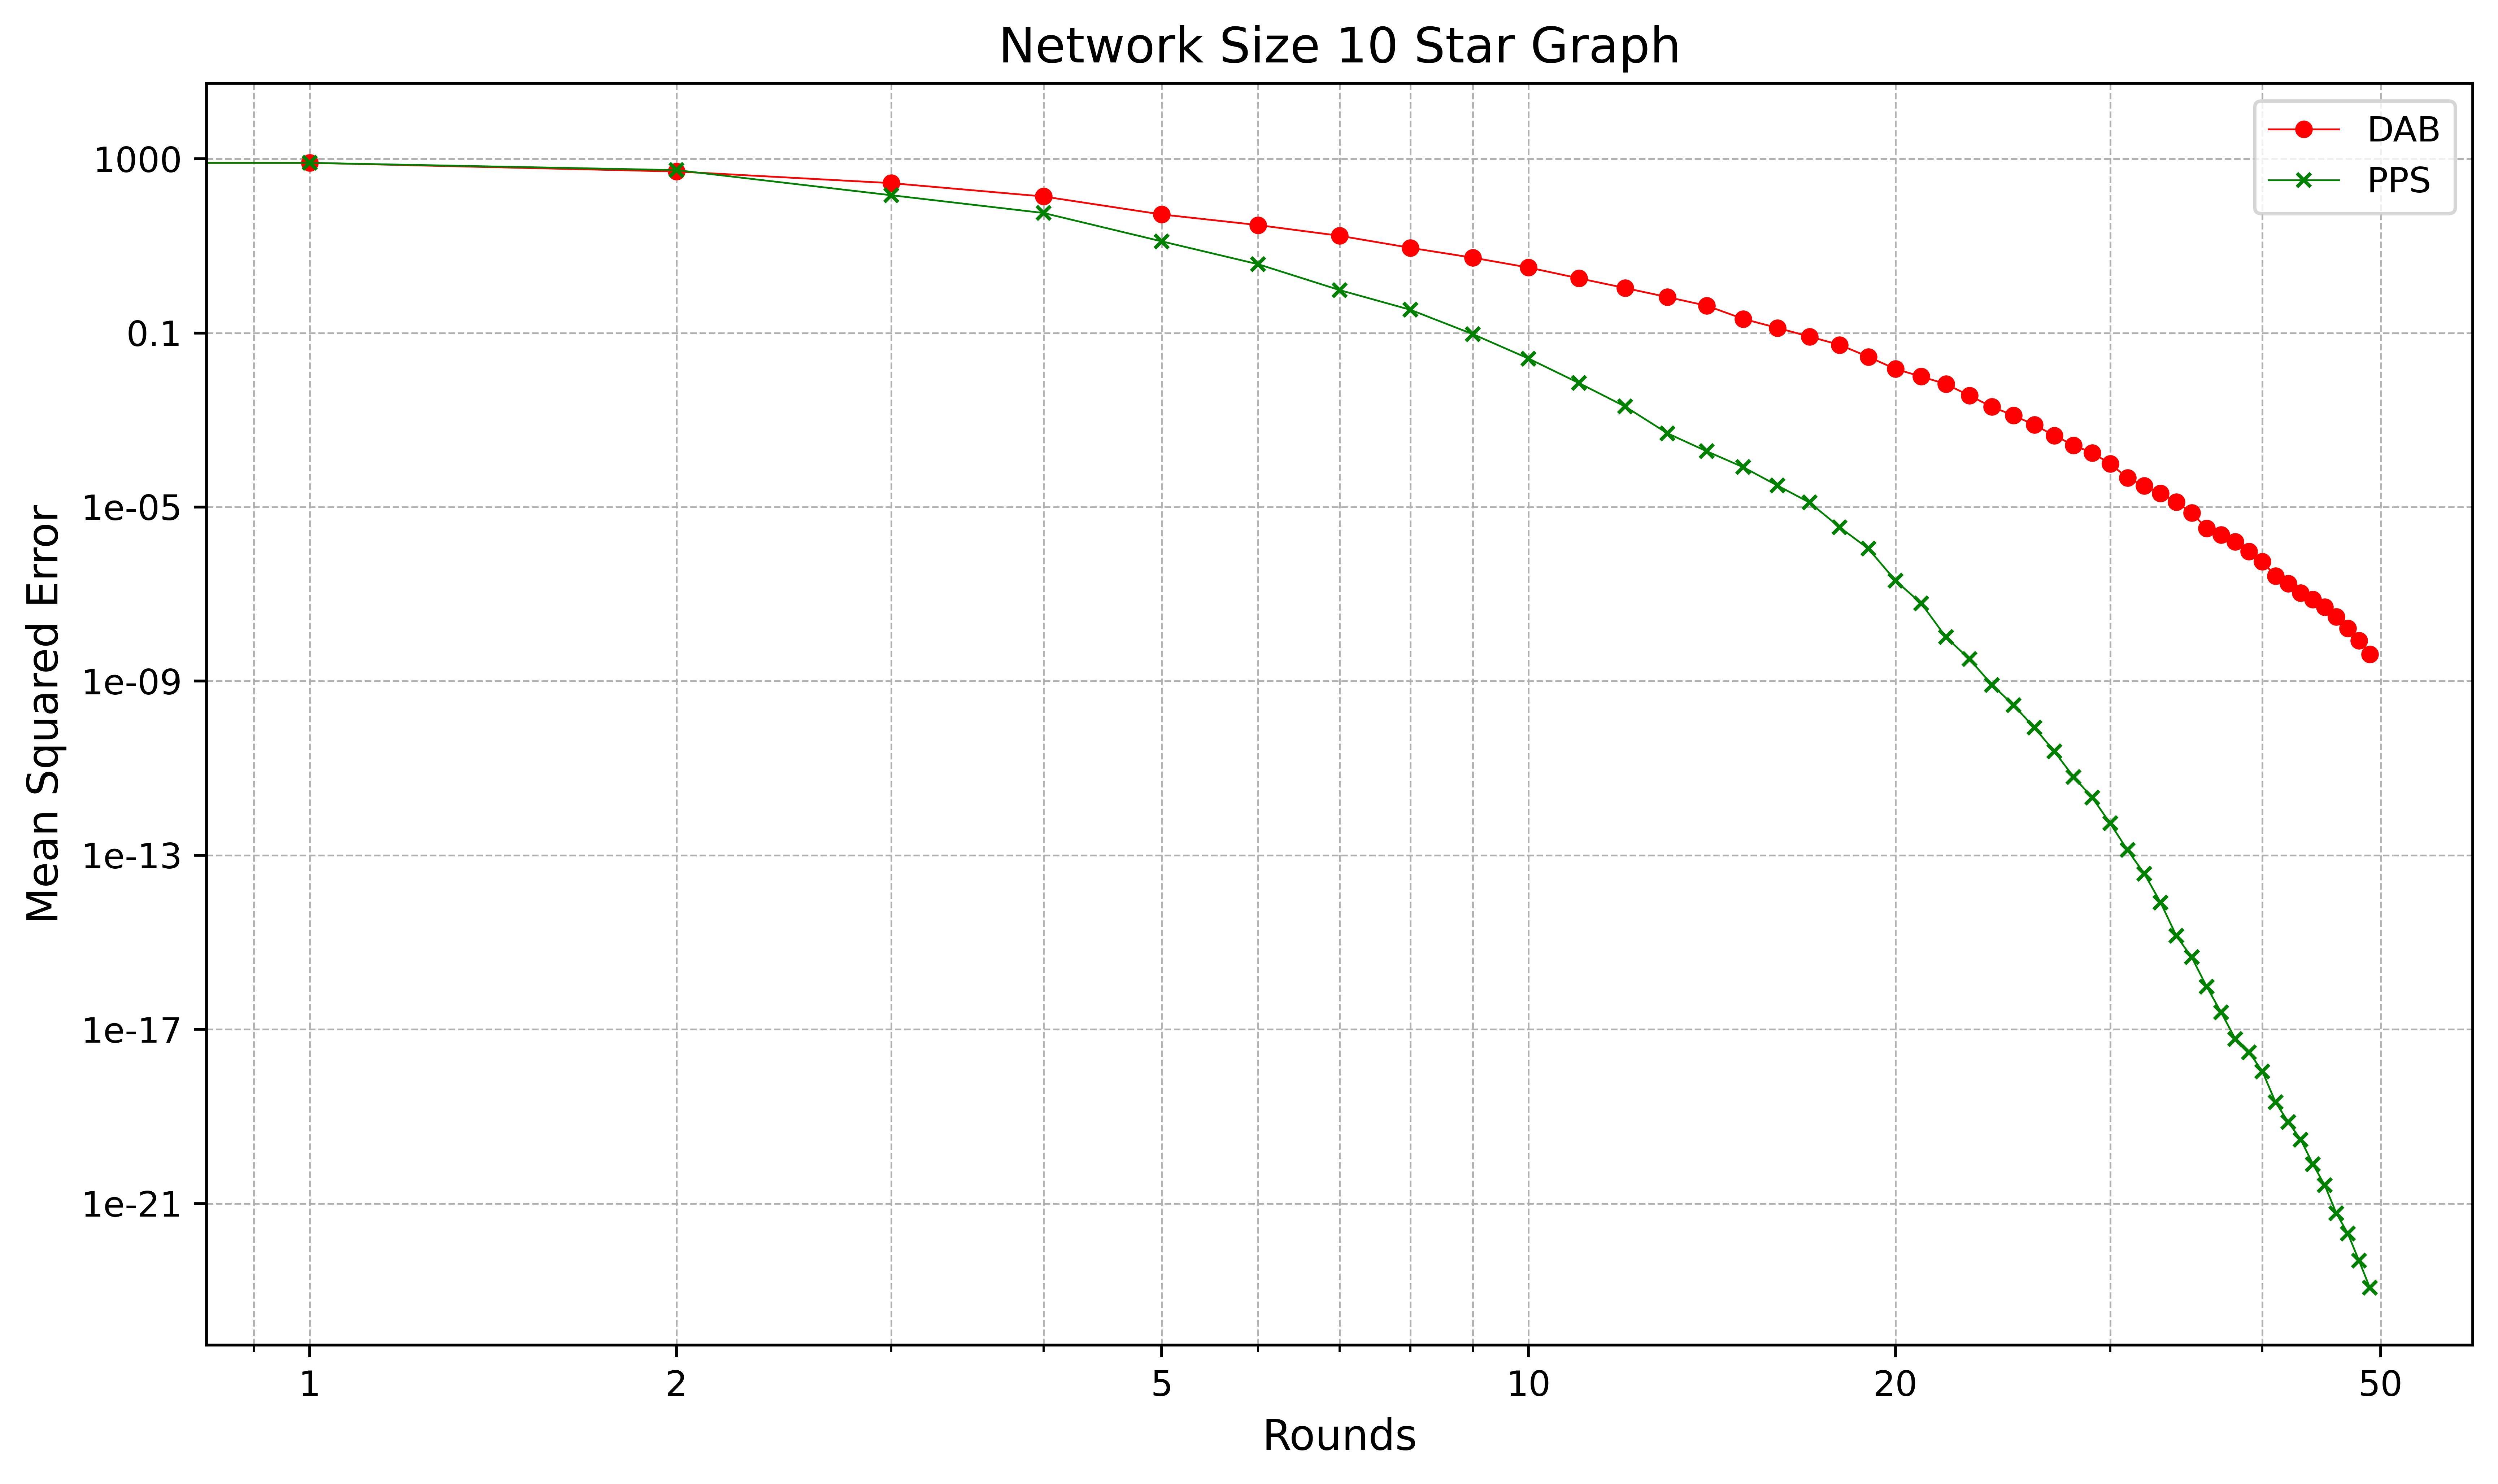
\includegraphics[scale=0.5]{figures/starGraphSimulations/DAB_vs_PPS_SG_r50_n10.png}
    \caption{Star graph: network size $10^{1}$ nodes}
    \label{fig:10StarGraph}
\end{figure}
\begin{figure}[H]
    \centering
    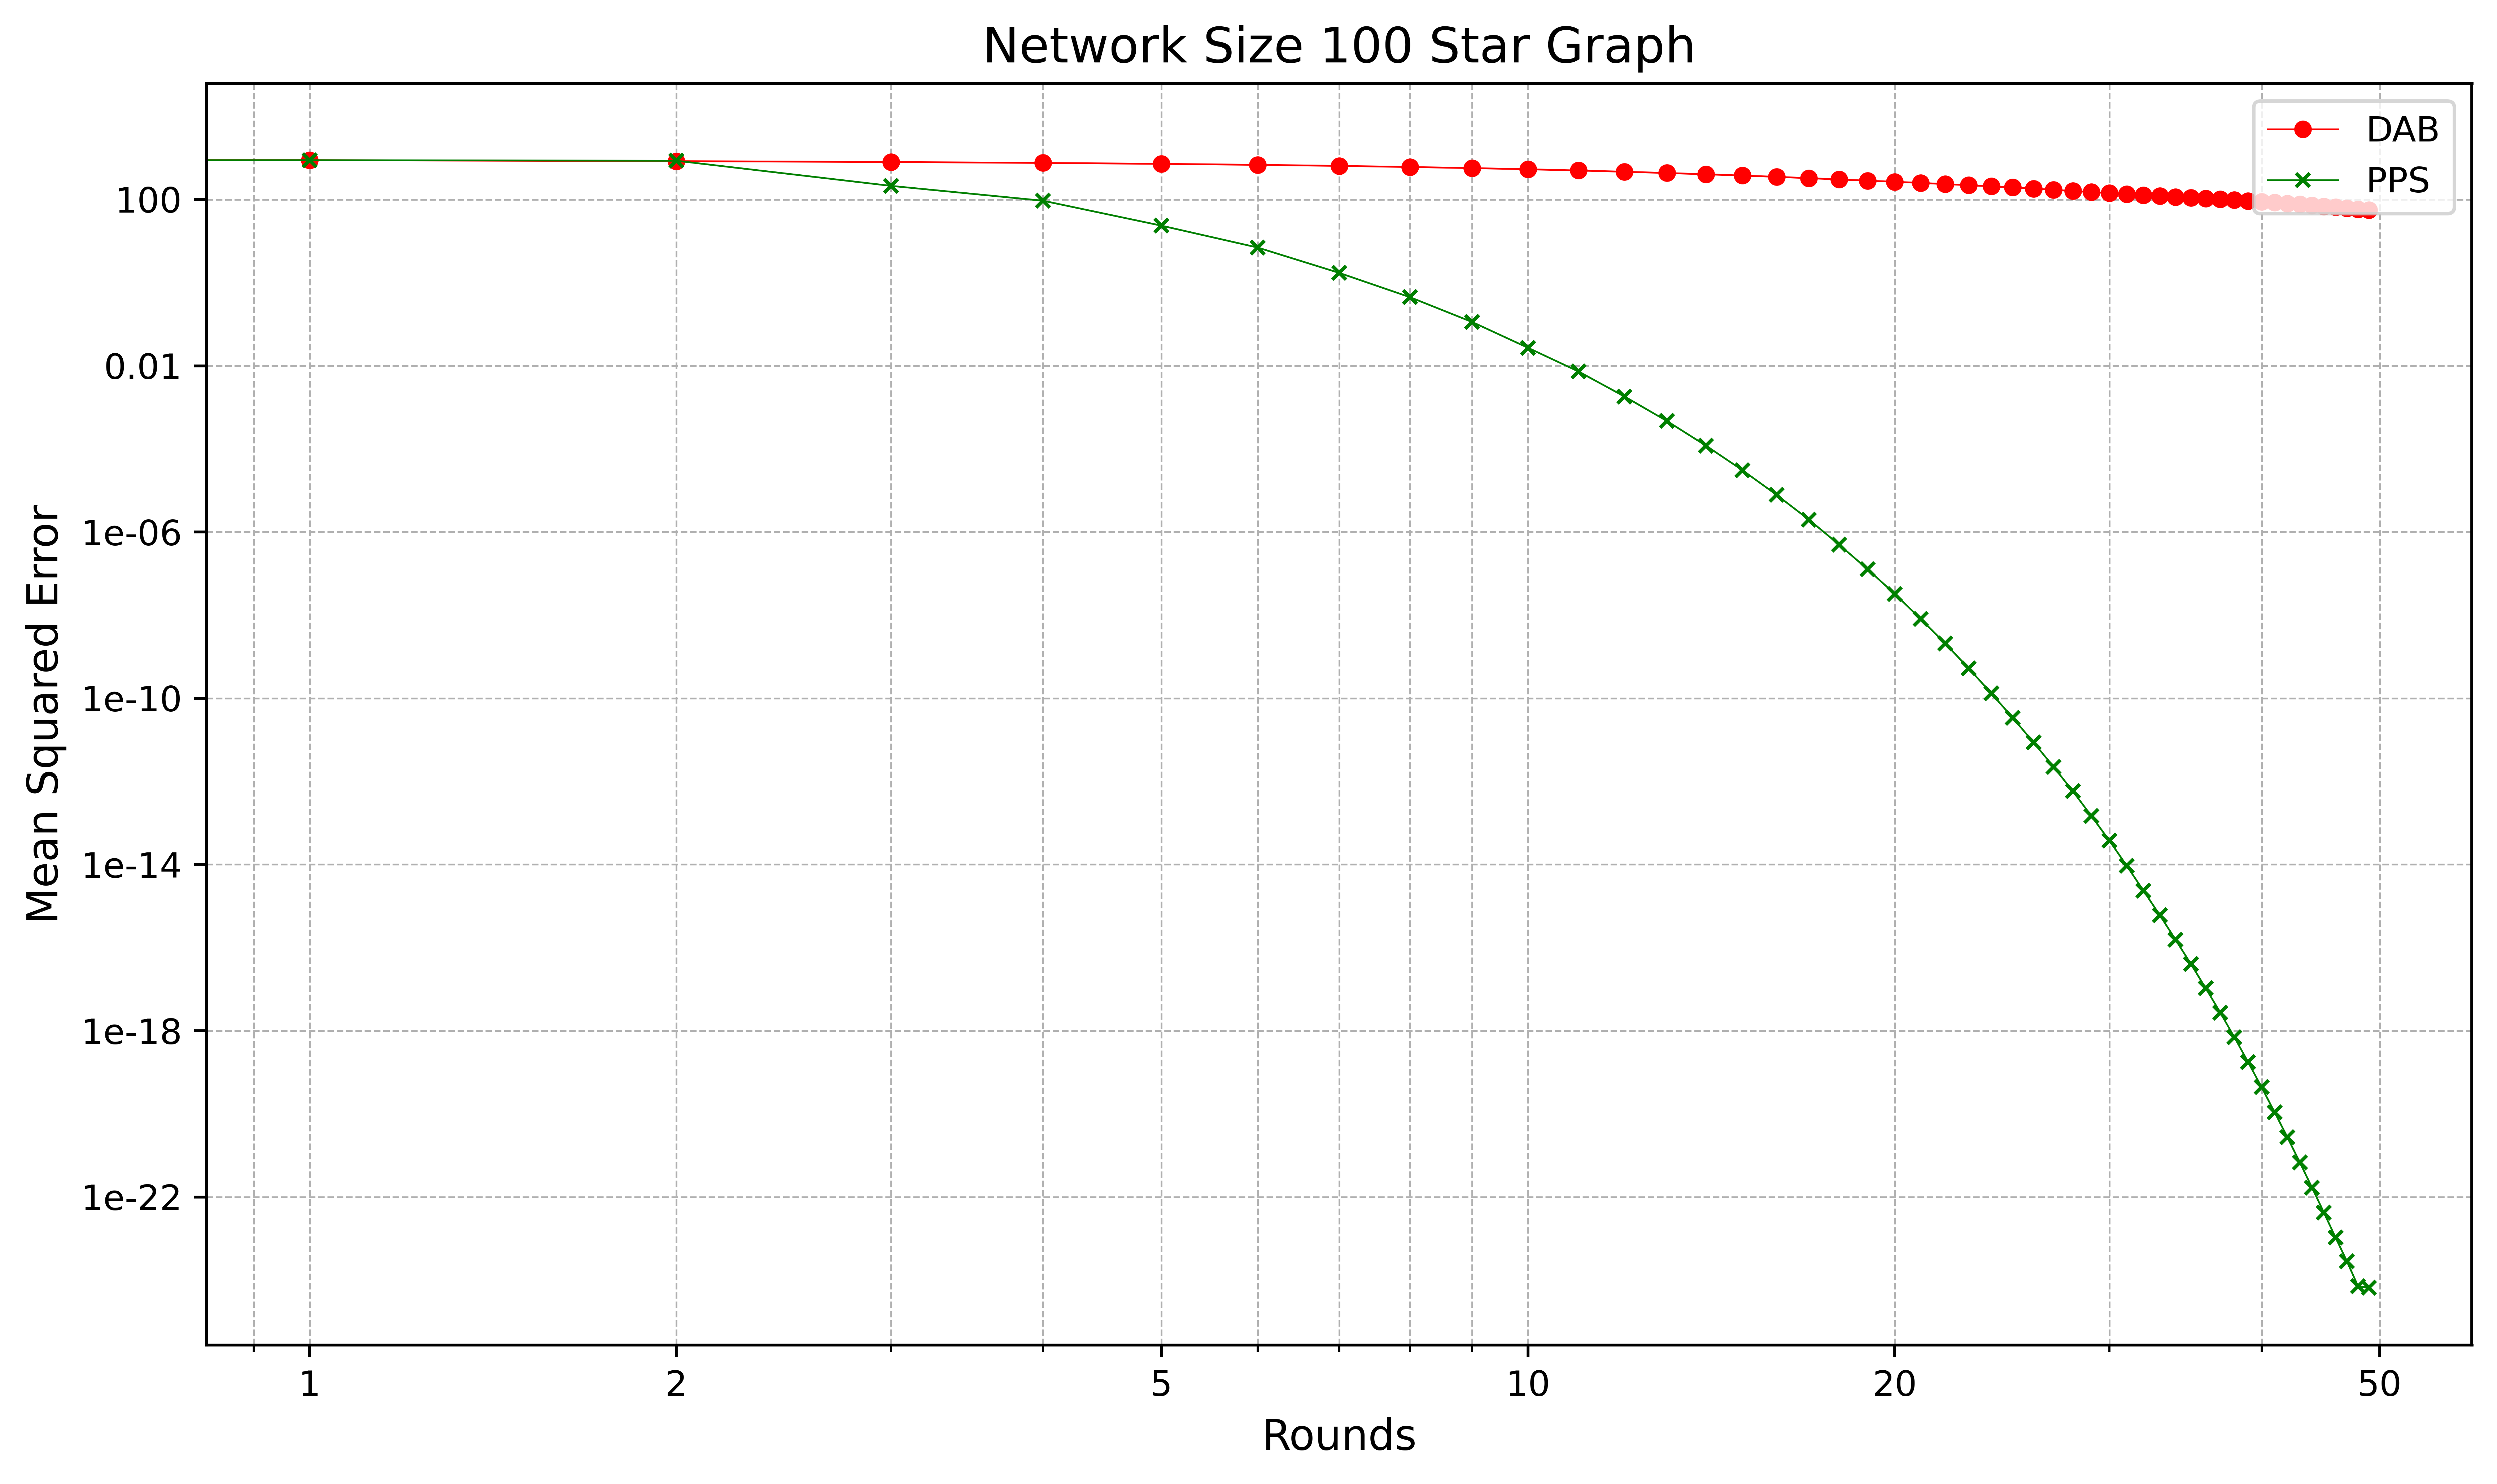
\includegraphics[scale=0.5]{figures/starGraphSimulations/DAB_vs_PPS_SG_r50_n100.png}
    \caption{Star graph: network size $10^{2}$ nodes}
    \label{fig:100StarGraph}
\end{figure}
\begin{figure}[H]
    \centering
    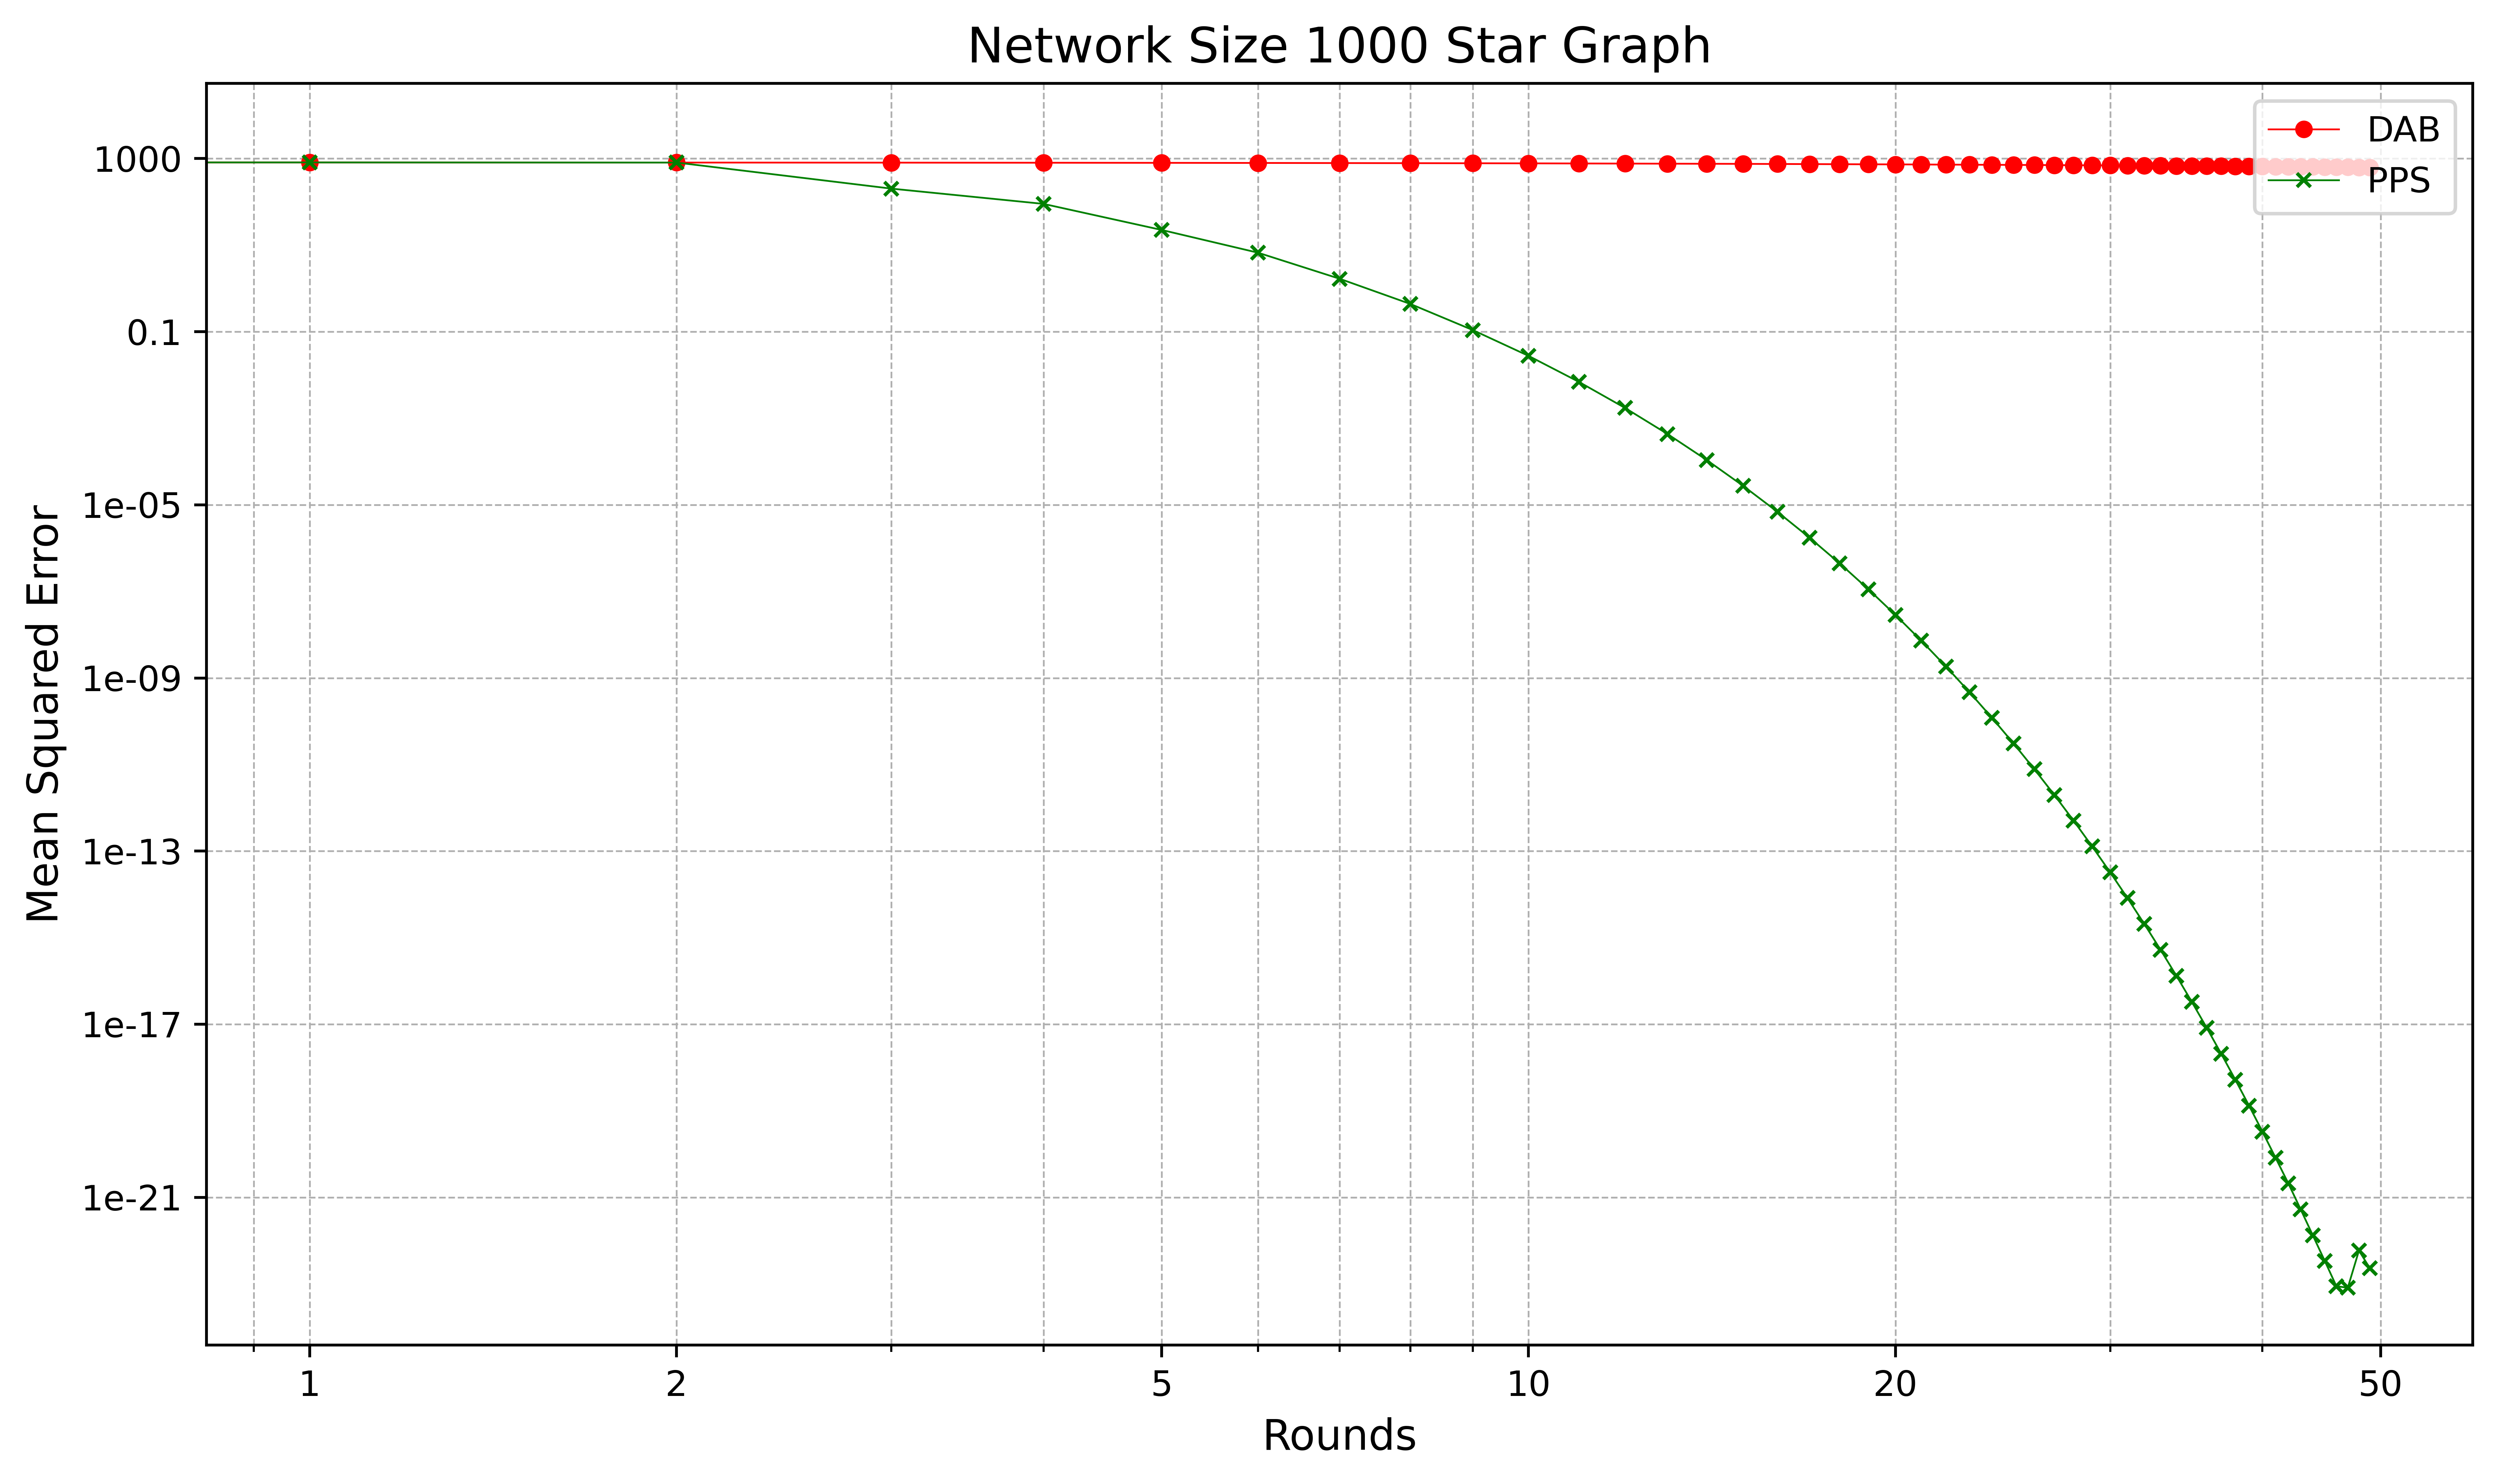
\includegraphics[scale=0.5]{figures/starGraphSimulations/DAB_vs_PPS_SG_r50_n1000.png}
    \caption{Star graph: network size $10^{3}$ nodes}
    \label{fig:1000StarGraph}
\end{figure}
\begin{figure}[H]
    \centering
    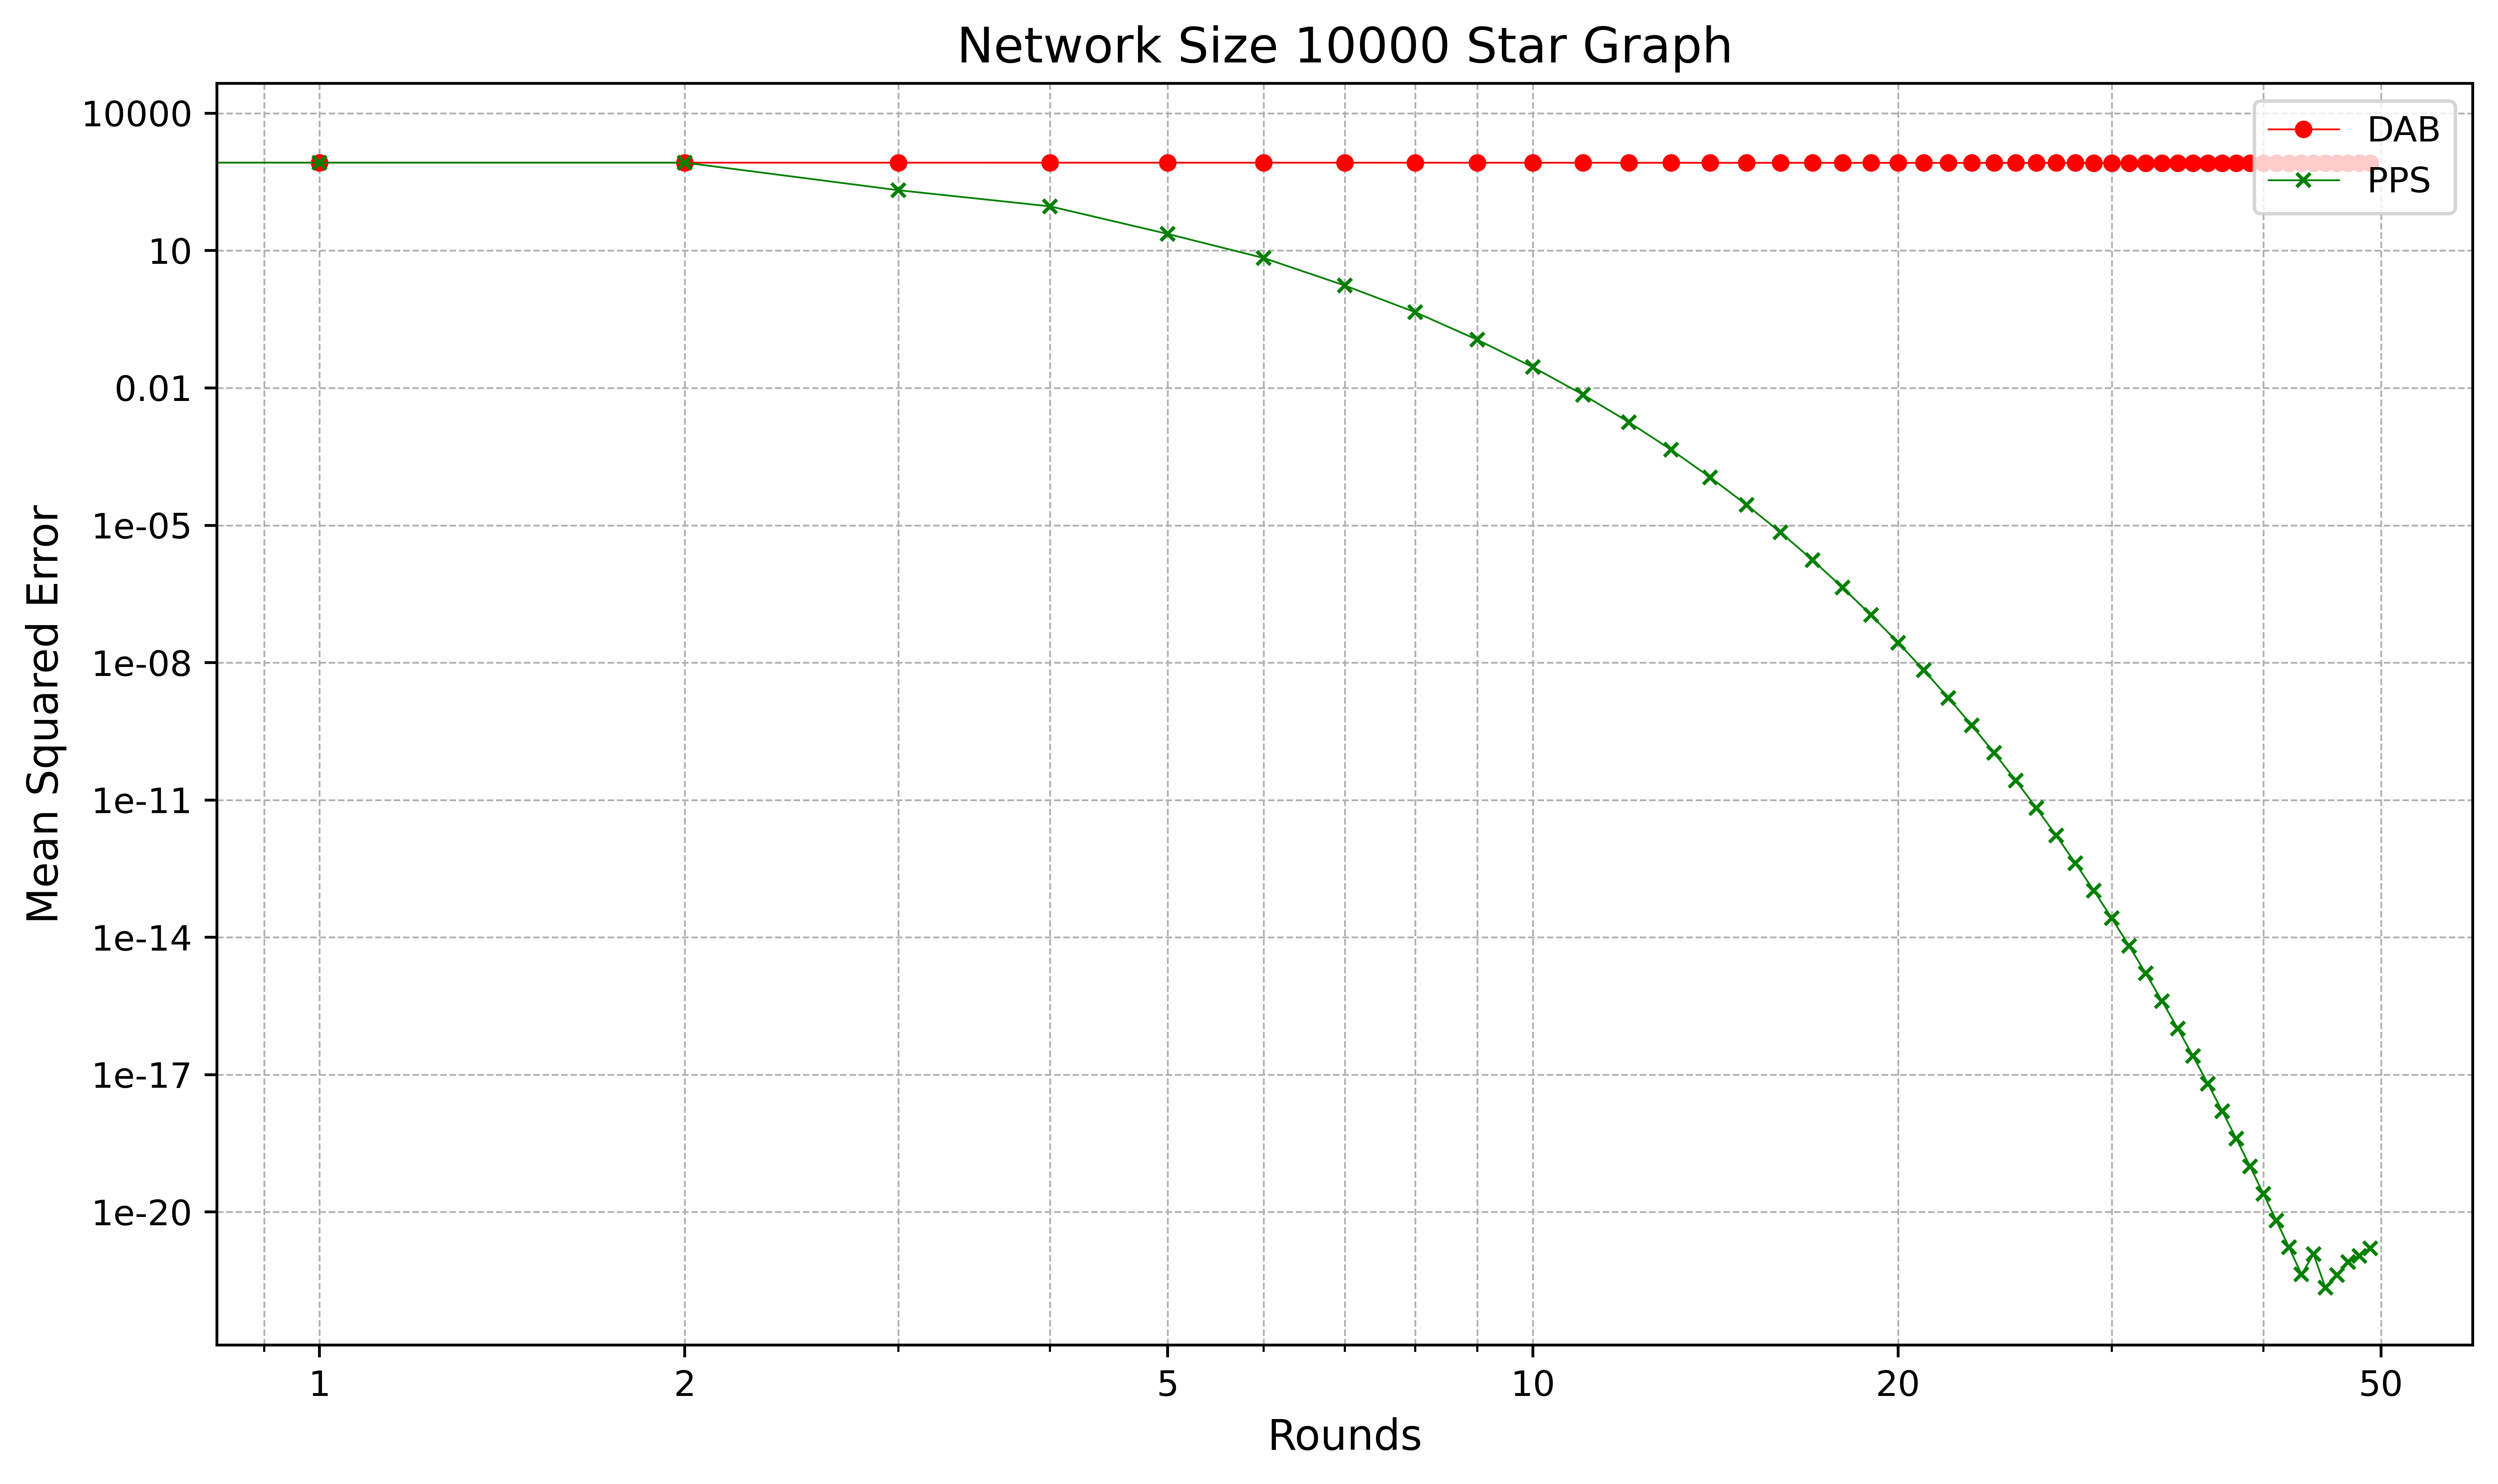
\includegraphics[scale=0.5]{figures/starGraphSimulations/DAB_vs_PPS_SG_r50_n10000.png}
    \caption{Star graph: network size $10^{4}$ nodes}
    \label{fig:10000StarGraph}
\end{figure}

\subsection{Closed Chain Graph}
\begin{figure}[H]
    \centering
    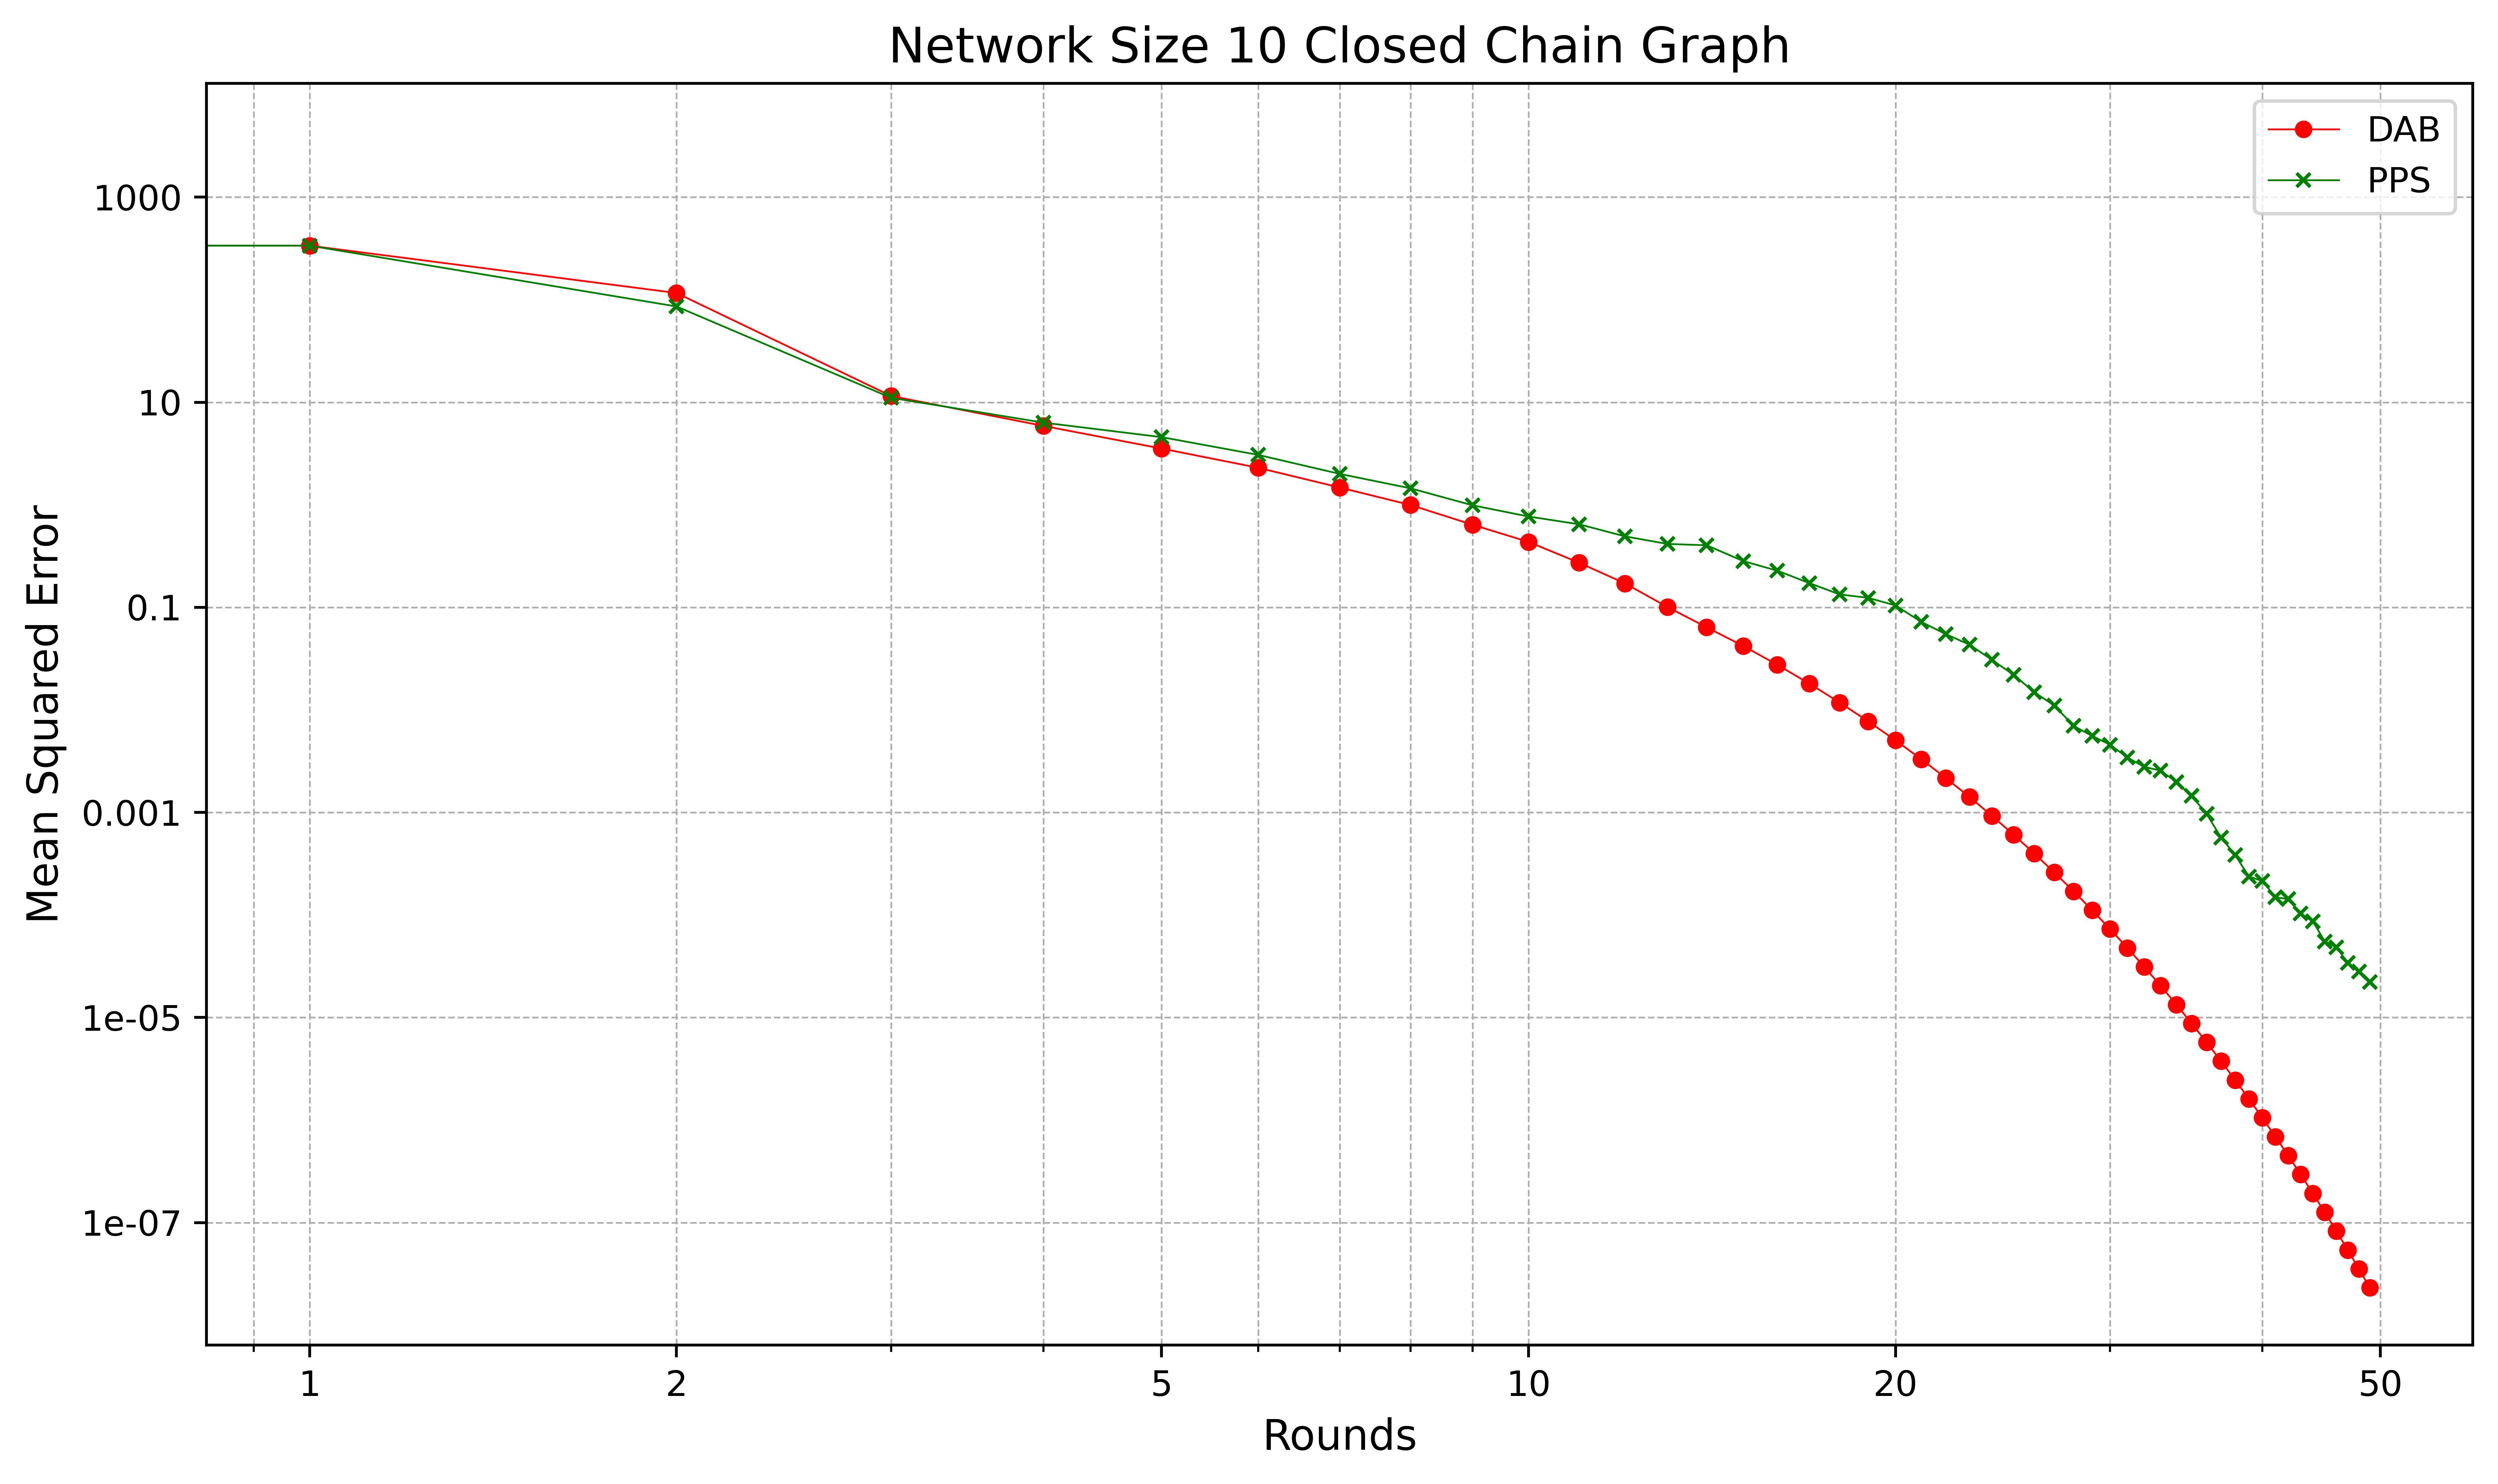
\includegraphics[scale=0.5]{figures/closedChainSimulations/DAB_vs_PPS_CCG_r50_n10.png}
    \caption{Closed chain graph: network size $10^{1}$ nodes}
    \label{fig:10ChainGraph}
\end{figure}
\begin{figure}[H]
    \centering
    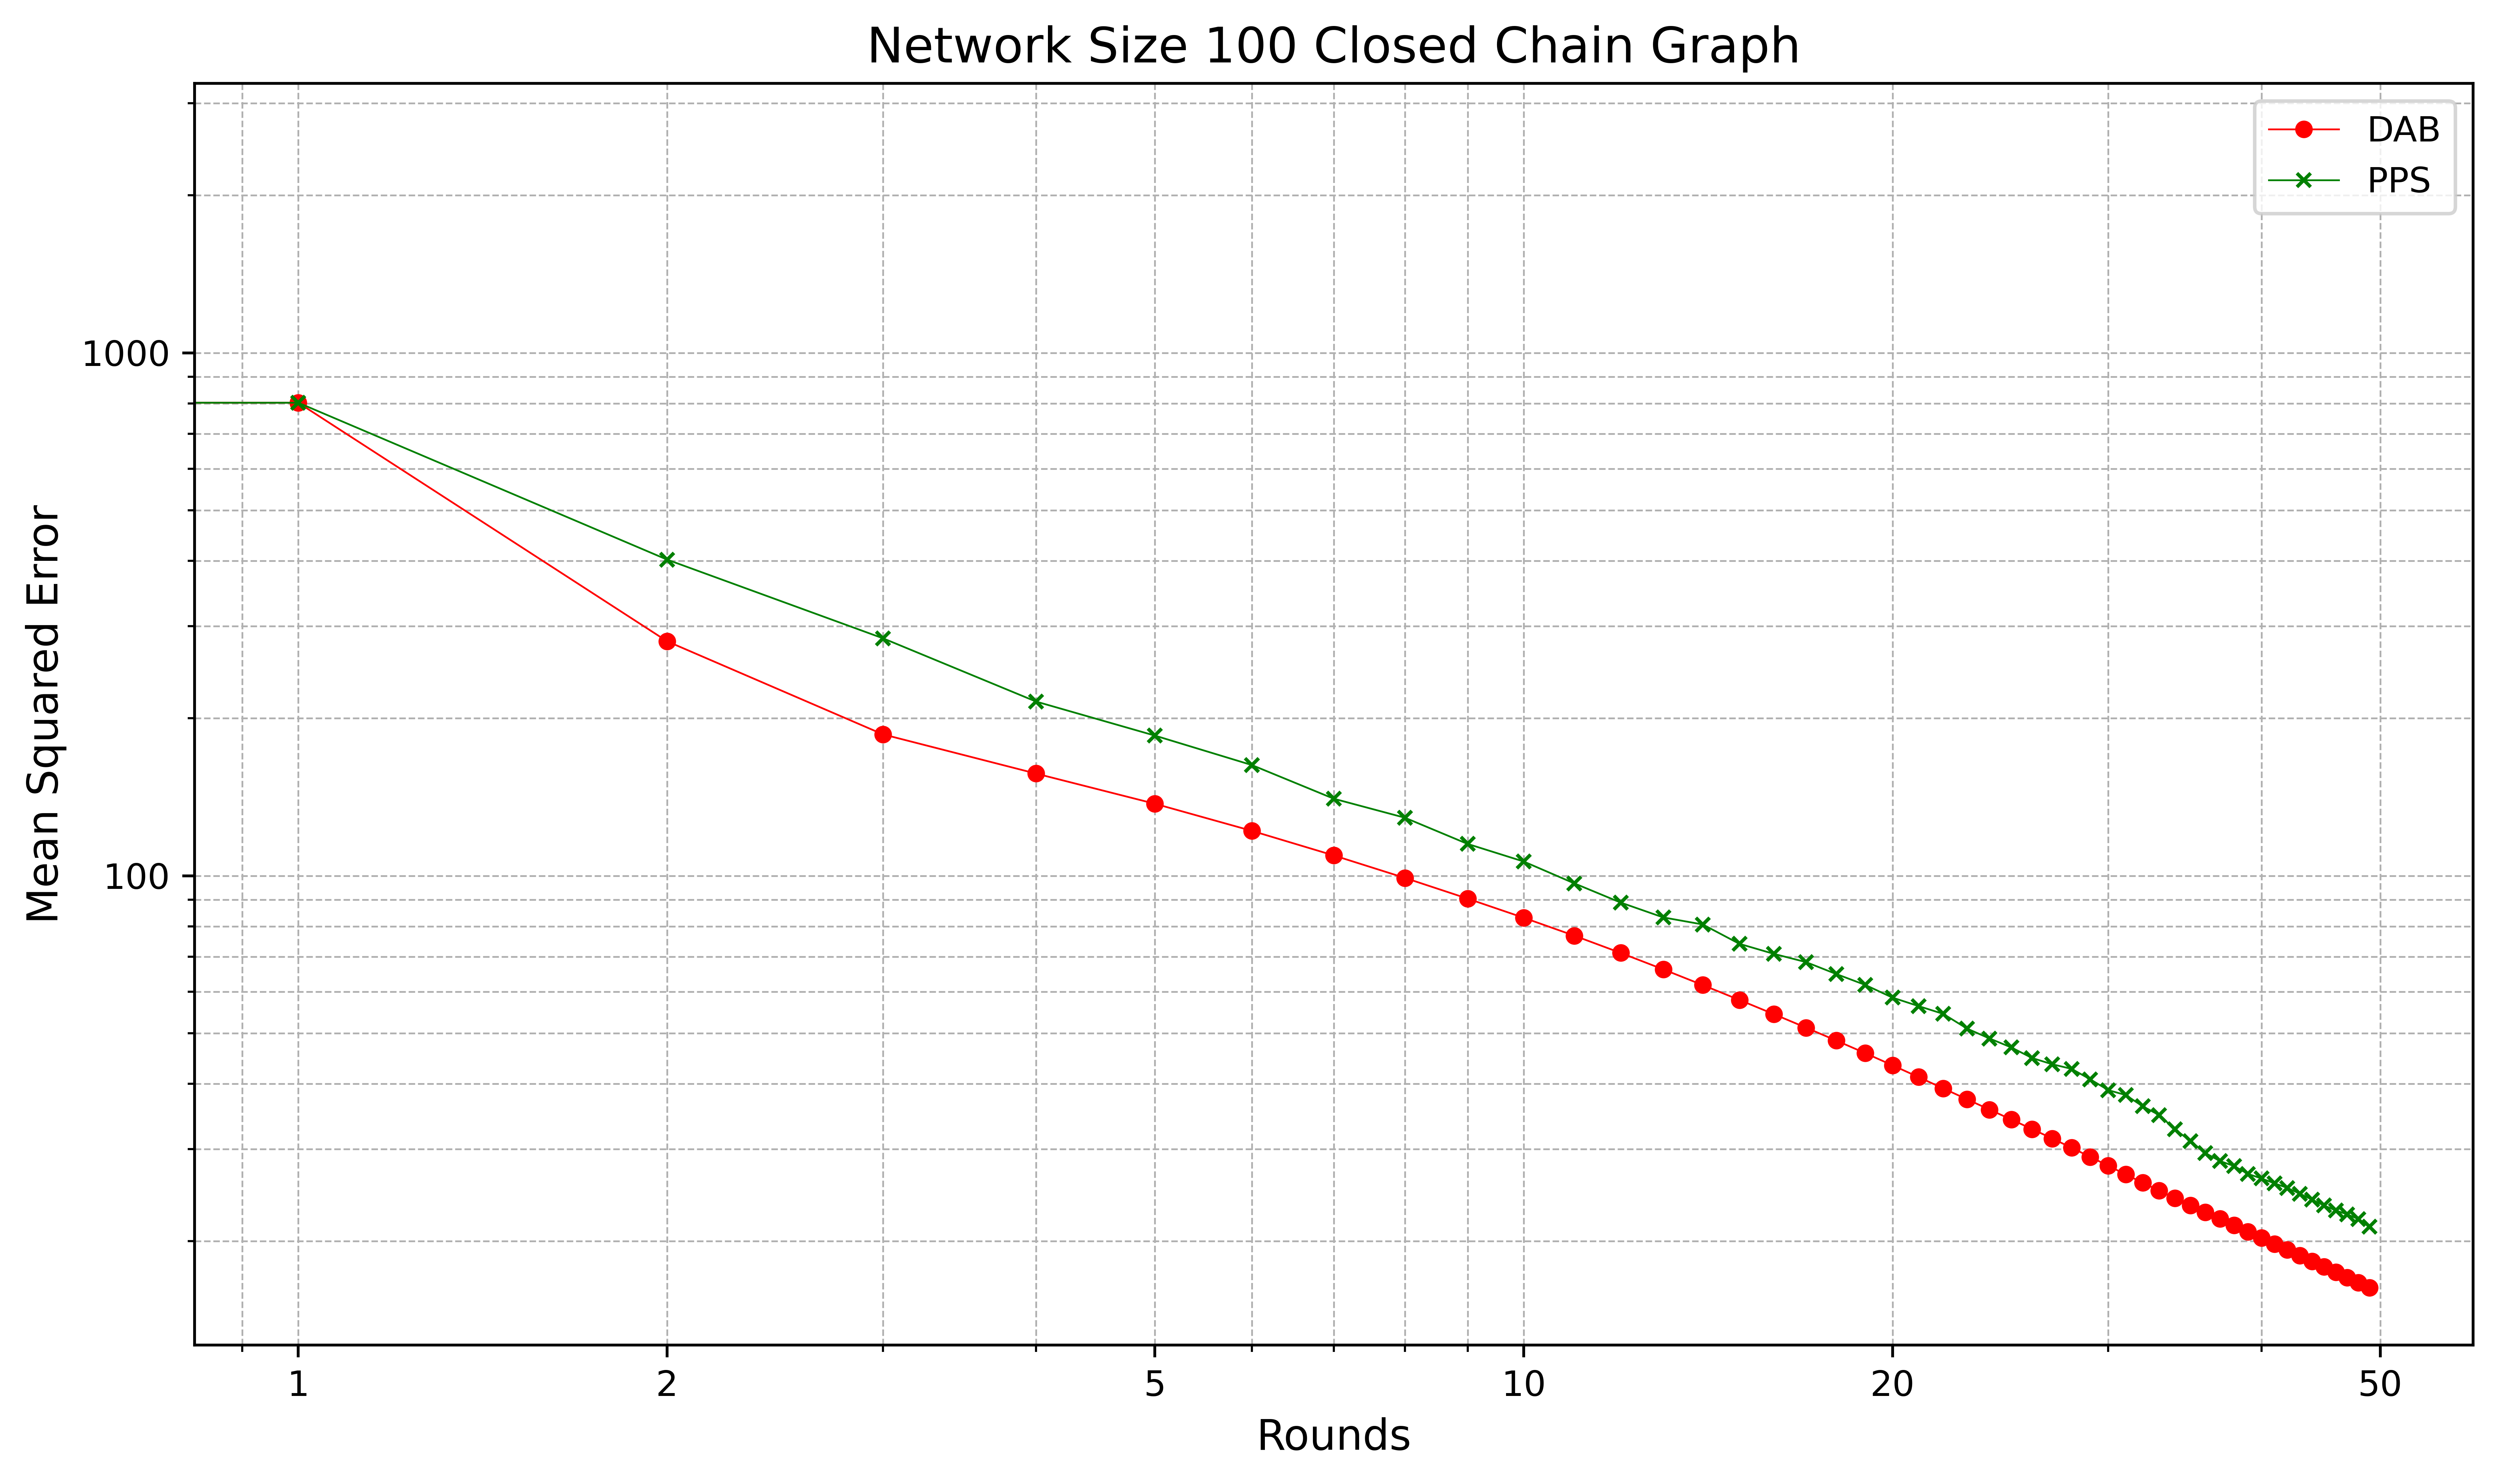
\includegraphics[scale=0.5]{figures/closedChainSimulations/DAB_vs_PPS_CCG_r50_n100.png}
    \caption{Closed chain graph: network size $10^{2}$ nodes}
    \label{fig:100ChainGraph}
\end{figure}
\begin{figure}[H]
    \centering
    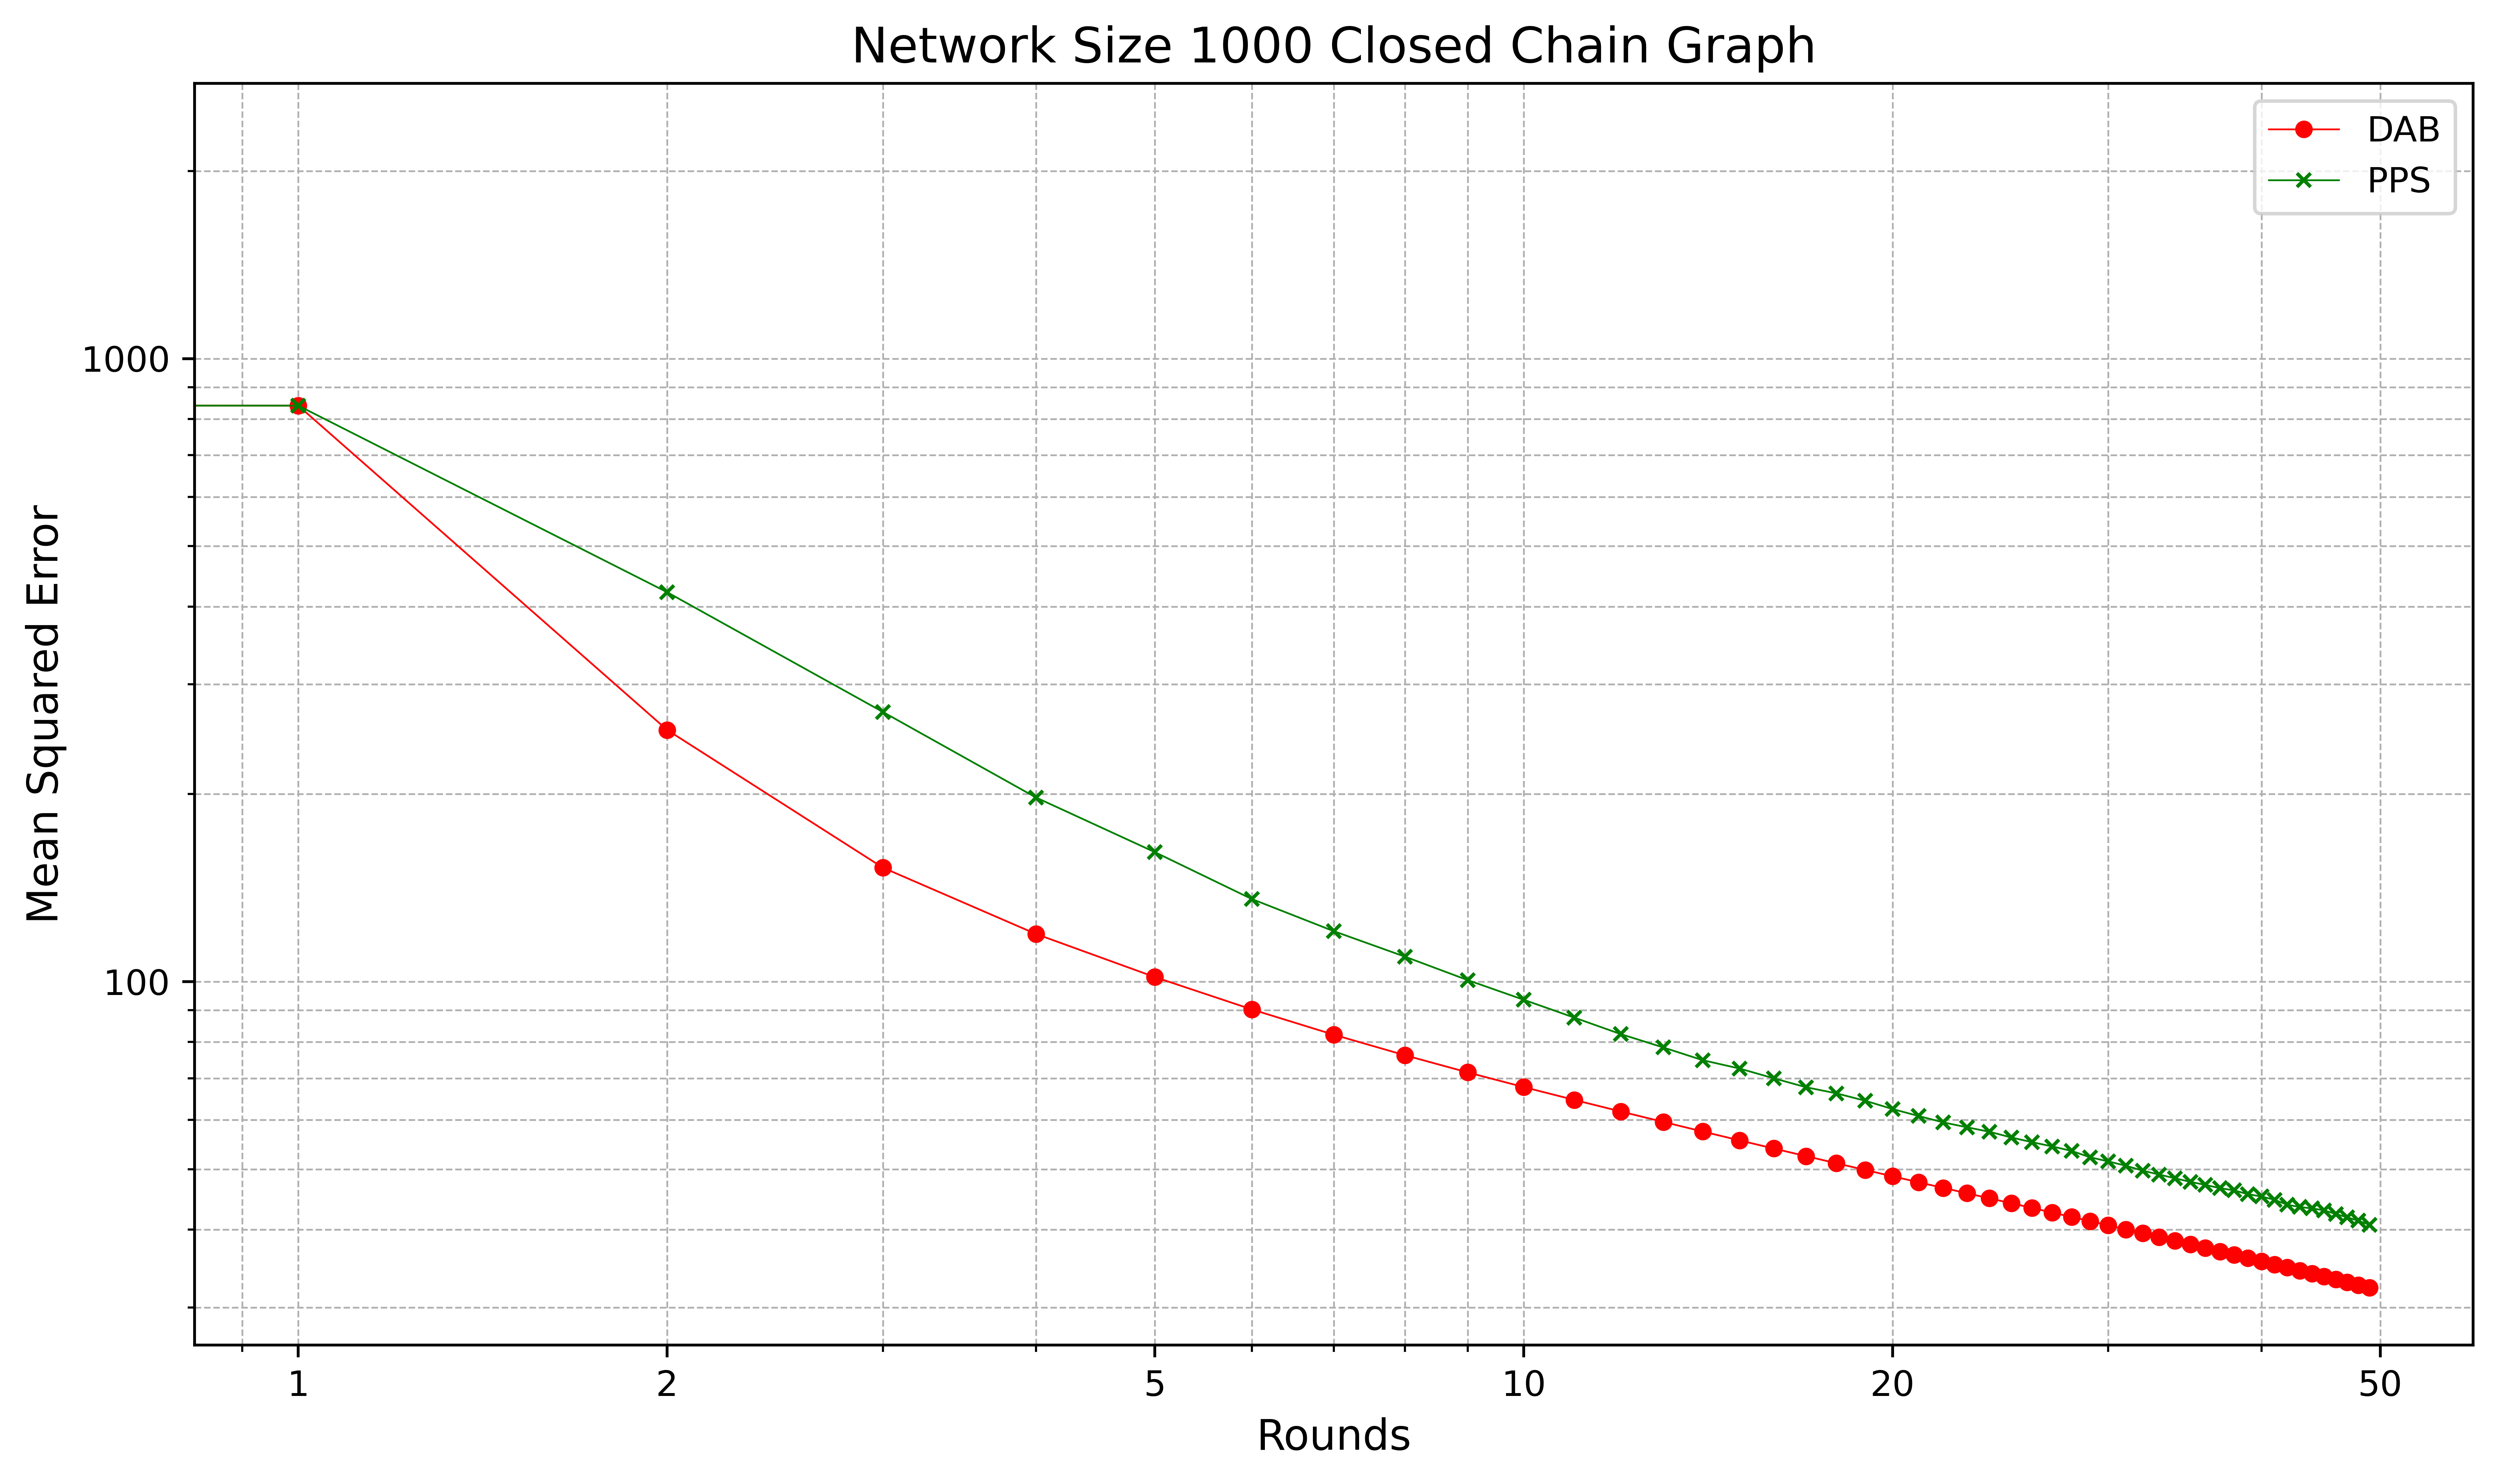
\includegraphics[scale=0.5]{figures/closedChainSimulations/DAB_vs_PPS_CCG_r50_n1000.png}
    \caption{Closed chain graph: network size $10^{3}$ nodes}
    \label{fig:1000ChainGraph}
\end{figure}
\begin{figure}[H]
    \centering
    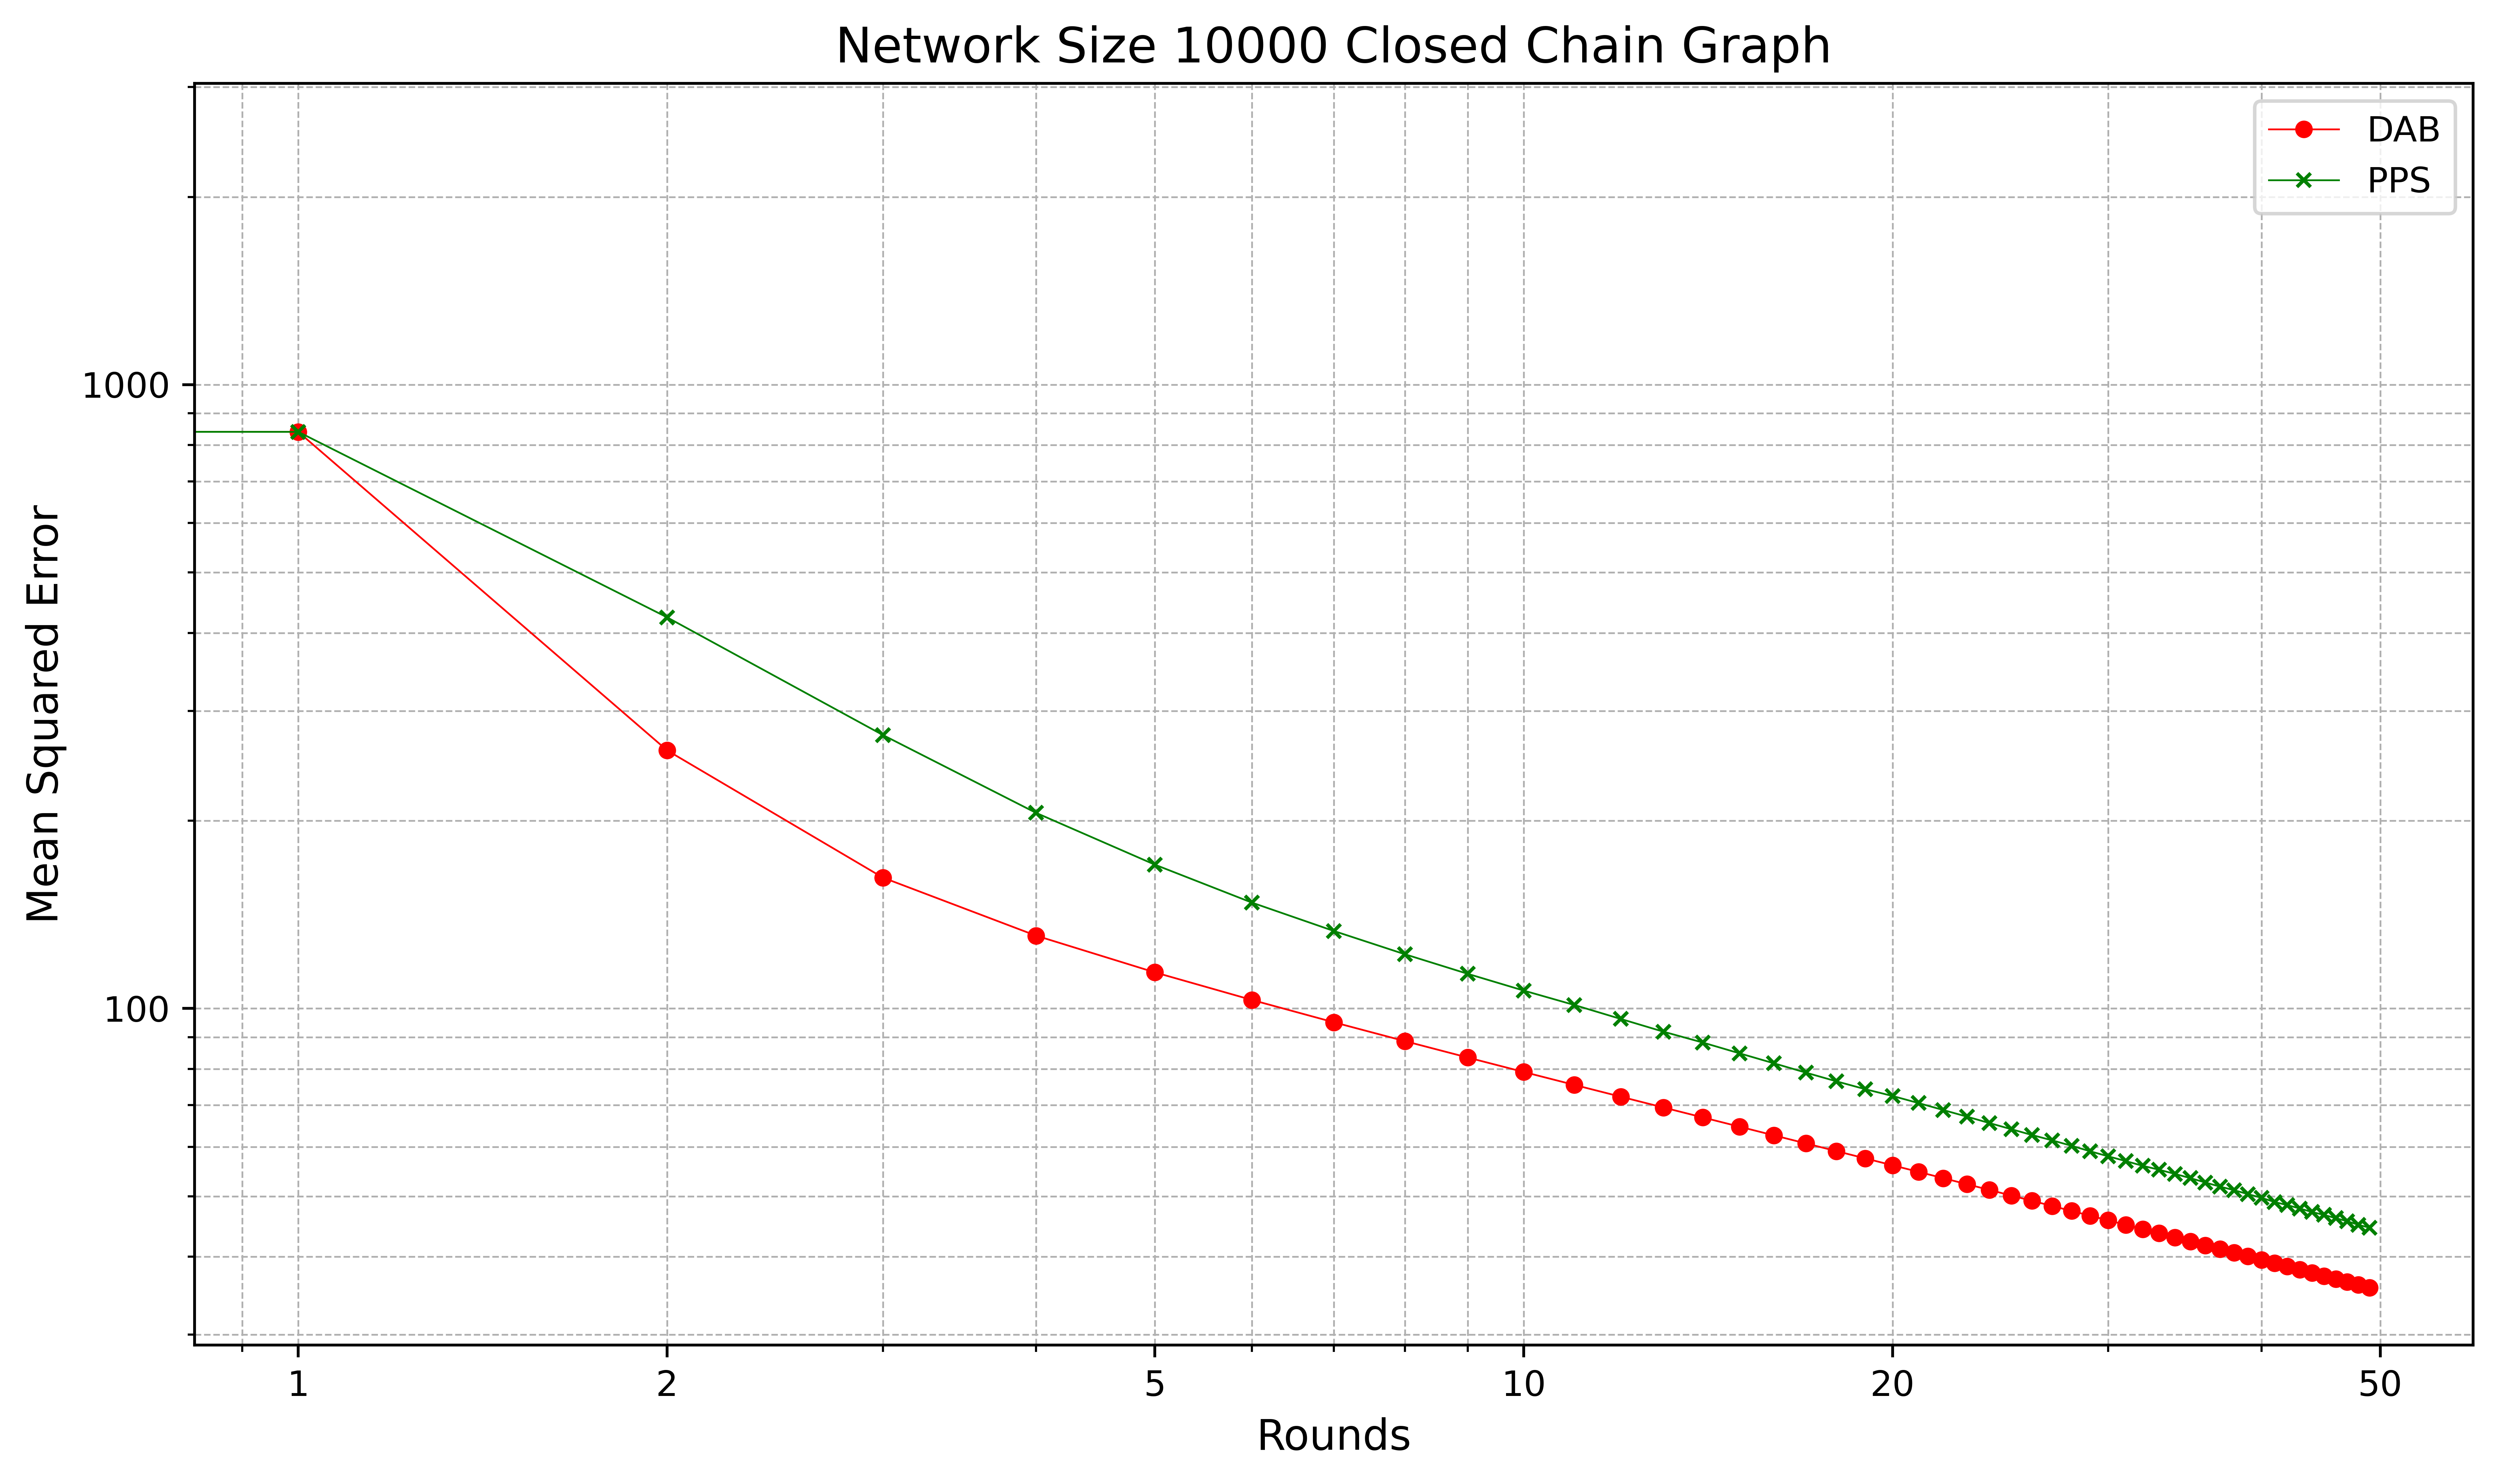
\includegraphics[scale=0.5]{figures/closedChainSimulations/DAB_vs_PPS_CCG_r50_n10000.png}
    \caption{Closed chain graph: network size $10^{4}$ nodes}
    \label{fig:10000ChainGraph}
\end{figure}

\subsection{Torus Grid Graph}
\subsection{Ring of Cliques}
\subsection{Lollipop Graph}
